
\newcommand{\mytitle}{The C64 PLA Dissected}
\newcommand{\myauthor}{Thomas 'skoe' Giesel}
\newcommand{\myemail}{skoe@directbox.com}

\providecommand{\documentheader}{\input{src/header_html.tex}}
\documentheader

\hypersetup{
    pdftitle = {\mytitle},
    pdfauthor = {\myauthor},
}

\begin{document}
\emergencystretch=0.15\hsize

%%%%%%%%%%%%%%%%%%%%%%%%%%%%%%%%%%%%%%%%%%%%%%%%%%%%%%%%%%%%%%%%%%%%%%%%
\thispagestyle{empty}
\begin{center}

\vspace*{2cm}
\textsc{\Huge \mytitle}\\[1cm]
{\large \myauthor}\\[3cm]

\begin{figure}[!htb]
    \centering
    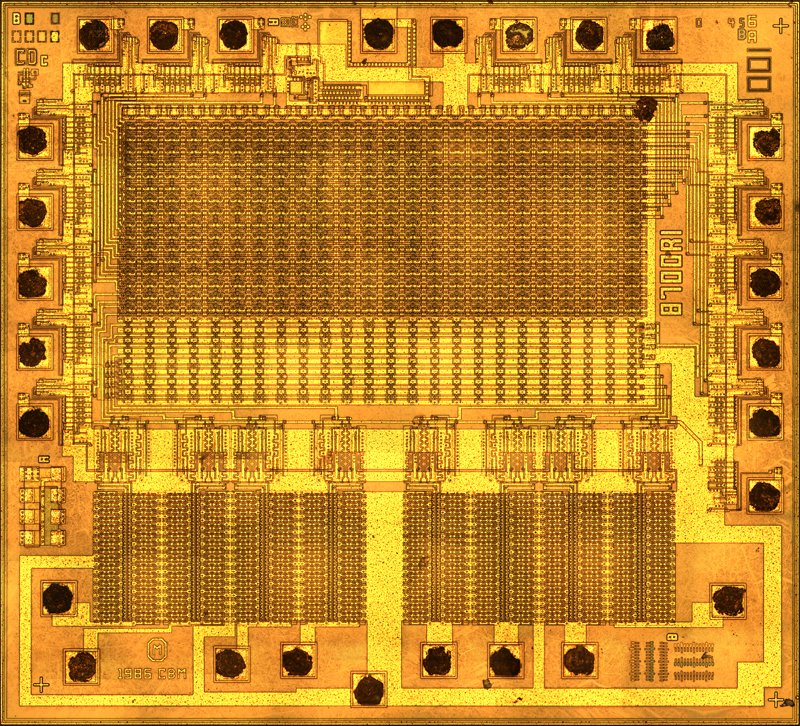
\includegraphics[width=0.8\textwidth]{8700R1s}
\end{figure}

\vfill

% Bottom of the page
{\large Revision 1.1, \today}\\[0.2cm]
\begin{figure}[!htb]
    \centering
    
\includegraphics[width=2cm]{cc-by-sa}
\end{figure}

\end{center}
%%%%%%%%%%%%%%%%%%%%%%%%%%%%%%%%%%%%%%%%%%%%%%%%%%%%%%%%%%%%%%%%%%%%%%%%

\pagestyle{plain}

\clearpage
\tableofcontents

\chapter{Introduction}

\section{Overview}

The programmable logic array (PLA) in the Commodore 64 (C64) is used to create
chip select signals from various other signals, e.g., from the current
address. These signals control which chip is to be connected to the data
bus. Therefore the PLA is responsible to implement the memory map of the C64.

If the PLA is broken, the CPU and the VIC-II\footnote{Video Interface
Controller II} direct memory access (DMA) can not access the right memory
and I/O devices anymore. In this case some chips can not be selected or more
than one chip is active at the same time. A total or partial malfunction of
the computer is the result. If a PLA is replaced with a part which does not
meet certain timing or electrical constraints of the chips connected to it,
the computer becomes unstable, possibly depending on temperature or hardware
extensions used or may refuse to work at all.

The logic implemented in the PLA defines the memory map. The logic equations
are described in chapter \ref{sec:logic}, among a short overview of previous
reverse engineering work related to it. Also the meaning of all signals
connected to the PLA for the working of the C64 is explained there. Appendix
\ref{sec:memmaps} contains the actual memory maps in a readable form as a
reference.

A list of PLAs found in C64s and measurements on some of them are shown in
chapter \ref{sec:hardware}. This chapter also describes which parameters are
important when a PLA is replaced with a different part. Most C64s shipped
with a PLA made by Commodore Semiconductor Group (CSG), better known under
their original name MOS Technology (MOS). A PLA of this type was opened,
photographed through a microscope and completely reverse engineered for this
article, down to the transistor level. Chapter \ref
{sec:mos-plas-inner-working} contains information about the inner workings
of the PLA, a redrawn chip layout and schematics. That chapter also contains
some background information by former Commodore/MOS engineers.

An actual implementation of a PLA replacement called \textit{realPLA} is
introduced in chapter \ref{sec:realpla} which can be built with parts being
in production at the time of writing. This implementation aims at highest
compatibility possible while using low-cost parts only. The design files for
the realPLA are available under a Creative Commons license.

Finally, chapter \ref{sec:conclusion} gives a conclusion about the findings
in this document. It also evaluates the compatibility of different PLA
replacements.

\section{About this Document}

Why is it necessary to write a document about the PLA in 2012? Information
already documented is spread over many articles, buried in old dusty books,
various forums and mailing lists, sometimes mixed with wrong statements.
Even though the PLA contains combinatorial logic only, it plays an essential
role in the C64 and other Commodore computers. ``The PLA's [...] were our
last salvation to pull a problem out of the fire, and our chance to impart
any coolness in logic,'' recalls Bil Herd, a former Commodore engineer.

Understanding the logical function of the PLA is important for programmers,
for hardware designers and for emulator developers. However, it is also
important to have a closer look at the electrical properties of the original
PLAs to implement a drop-in replacement for PLA chips. This document
addresses both topics.

This document collects information already documented and adds new
measurement and research results. The text and all figures are licenced
under Creative Commons Attribution-ShareAlike 3.0 Unported (CC BY-SA 3.0).


\section{Acknowledgements}

I wish to thank the engineers of Commodore for the interesting memory maps
achieved by using the PLA. Unfortunately you forgot a KERNAL cartridge ;)

Furthermore I would like to express respect to all persons who examined the
PLA before and published their results, namely William Levak, Jens
Schönfeld, Marko Mäkelä, Andreas Boose and Mark Smith.

All PLA logic incorporated in this document and used for the implementation is
based on the JEDEC file by Raymond Jett of arcadecomponents.com. It was
created by reading a C64 PLA with a TopMAX programmer and Max Loader
software. The file is available at \cite{AC12} and in the source code
repository of the realPLA implementation \cite{realPLA12}.

Segher Boessenkool described in a mail to the cbm-hackers mailing list
\cite{Boess12} how the JEDEC file can be read directly. Thanks to his
explanation I was able to implemented a small tool which converted the JEDEC
file to VHDL equations directly. Segher also helped me much with the
first steps to learn to read NMOS die shots and also reviewed this document.

The micrographs for this document were made by Dr. Martin `enthusi' Wendt
(8700R1) and Philipp `Dexter' Maier (7700R2). AREA51HD donated the chips we
used for that.

Gerrit Heitsch, TheRyk and Björn `JMP\$FCE2' Wieck sent some different PLAs
for the investigations. Gerrit also gave some valuable hints for various topics
and Björn made some additional measurements. Ingo Korb helped with proofreading.

Last but not least I also want to thank the former Commodore engineers
Bil Herd, Bret Raymis, Dan Morris, Dave DiOrio, Dave Esposito and James
Redfield for interesting background information and for clarifying some
technical issues.

All quotes in this document which do not state a reference are taken from
personal communications with the persons concerned.

\newpage
\section{Document Revisions}

Please look out for new revisions of this document. If you have new or
additional information relevant for this document or found mistakes, please
contact me. The latest version of this document is available at
\url{http://skoe.de/docs/c64-dissected/pla/}. Feel free to mirror these files.

\begin{table}
\begin{minipage}{\linewidth}
    \tabletextsize
    \centering
    \begin{tabularx}{\mywidthfull}{l|X}
        \toprule
        Revision & Changes \\
        \midrule
        1.0 & Initial release \\
        1.1 & Minor changes after review comments;
              link to Jens Schönfeld's PLA tool added; SuperPLA V3 mentioned \\
        \bottomrule
    \end{tabularx}
    \caption{Document Revisions}
    \label{tab:docrevs}
\end{minipage}
\end{table}


\chapter{The Logic in the PLA}
\label{sec:logic}

\section{The Development}

The logic needed to get the C64 running was programmed by Bob Yannes. ``He
just needed some glue logic to tie everything together,'' recalls James
Redfield. According to Bil Herd, ``[The original PLA terms] appear on an
82S100 worksheet photocopied out of the Signetics databook.''

\section{Reverse Engineering History}

The memory maps in the Programmer's Reference Guide \cite{PRG83} show all
possible configurations as they are seen by the CPU, including Ultimax mode.
However, some details cannot be taken from that book, especially memory
configurations for VIC-II accesses.

Probably the earliest full reverse engineering of the logic programmed to
the PLA was written by William Levak in 1986. It was published in The
Transactor magazine \cite{Lev86}. He read out a PLA, put the binary dump
onto a disk and used a computer program to extract the logic table from it.
Using this way he avoided transcription errors. He double-checked the results
against two other PLAs. Unfortunately the article in The Transactor has
some typesetting mistakes in the memory maps, although the logic table is
correct and nicely optimized.

Some years later, in 1994, Jens Schönfeld - apparently not aware of William's
work - captured the truth table again. He, Marko Mäkelä, Andreas Boose and
others \cite{PLA95} investigated that table and derived equations from
it. Mark Smith took a programmer and read out an 82S100 in 1995. The results
confirmed their work.

\section{PLA Logic Revisions}

Very early C64s contain a PLA which was labeled \textit{REV2 7E17}. This
version is said to have a different logic implemented. Unfortunately no
binary or JEDEC dump was available for this document. The next version was
\textit {REV3 8411}. The four digit hex number is the checksum of the
original JEDEC file most likely.

Different PLAs with different part numbers by different manufacturers found
in C64s have been read out. The logic in all of them was identical
with REV3, so this was the final revision.

\section{How the PLA is Connected in the C64} \label{sec:connection}

To understand the logic in the PLA, first let's have a look how it is
connected in the C64. All descriptions are based on the schematic \#251138 from
\cite{Serv85}, but apply for other C64 models too.

\subsection{\#CAS (I0)}

The input line I0 is connected to the \#CAS output of the VIC-II. In every
Phi1 and Phi2 cycle this line is pulled down by the VIC-II to initiate a
read or write access to DRAM. Depending on the other inputs, the PLA may
propagate the \#CAS pulse to the \#CASRAM output or mask it out. Only if it
is propagated to \#CASRAM, DRAM is actually addressed by the memory access.
When \#CASRAM remains high in a cycle because it is disabled by the PLA
logic, the DRAM access is rendered ineffective, or more precisely it turns
to a RAS-only refresh cycle.

\subsection{\#LORAM, \#HIRAM, \#CHAREN (I1 to I3)}


The lines \#LORAM (I1), \#HIRAM (I2) and \#CHAREN (I3) are connected to the
processor port of the CPU, better known as bits 0..2 of \$00/\$01 in the
6510/8500. After a reset these lines are all set to input mode by the CPU,
which means that they are not driven. To make sure the have a sane value
when the machine is started, they are pulled up by R43, R44 and R45. With
all these values being 1, the C64 can start with KERNAL, I/O and BASIC
banked in.

\subsection{\#VA14 (I4)}

\#VA14 (I4) is one of the additional video address lines for the VIC-II. The
VIC-II has a 14 bit wide address bus to address 16 KiByte of memory, while
the C64 has 64 KiByte of DRAM. To allow the VIC-II to address any of the
four 16 KiByte chunks available in these 64 KiByte, two additional address
lines called \#VA14 and \#VA15 are generated by programmable outputs of the
CIA U2. They are fed to an extra address multiplexer U14. This is a 74LS258,
which has inverted outputs.

The I/O ports are in input mode after the CIA has been reset. In this case
these two lines are pulled high by internal pull-up devices in the CIA,
which effectively selects bank 0 on startup. Note that these two video
address bits do not appear on the global C64 address bus, they are only used
for DRAM accesses. \#VA14 is also connected to the PLA to influence the
character set ROM mapping.

\subsection{A15 to A12 (I5 to I8)}

The address bus lines A15 to A12 (I5 to I8) are connected to the global
address bus. They are driven by the CPU when AEC from the VIC-II and \#DMA
from the Expansion Port are both high. During VIC-II cycles, when AEC is
low, they are pulled up by RP4. When they are pulled up by this resistor
array only, it is possible to change them from the Expansion Port. These
address lines are used by the PLA to control the memory mapping when AEC is
high, i.e. during CPU cycles. However, they are also evaluated in the PLA in
Ultimax mode when AEC is low, which makes an interesting trick possible,
shown in section \ref{sec:vic-memory-config}.

\subsection{BA (I9)}

BA (I9) is set low by the VIC-II when it wants to halt the CPU to be able to
use both half-cycles to get more memory bandwidth. When the VIC-II pulls
down BA to take over the bus, there are three cycles left for the CPU. In
these cycles up to three write accesses can take place, which is the maximum
number of consecutive write accesses a 6510 does. However, the CPU stops its
work before the first read access is started.
Therefore there are up to three dummy read accesses on the bus until the
VIC-II takes over control.

\subsection{\#AEC (I10)}

\#AEC (I10) is an inverted version of AEC. \#AEC is high whenever the VIC-II
is going to control the address bus. This is the case in every Phi1 cycle
and in all full cycles when is BA low, after the CPU got three extra Phi2
cycles.

\subsection{R/\#W (I11)}

The signal R/\#W (I11) is high for read accesses and low for write accesses.
Note that it is pulled up with resistor R51, because this line is not driven
by the CPU when AEC or \#DMA are low.

\subsection{\#EXROM, \#GAME (I12, I13)}

The two lines \#EXROM and \#GAME can be pulled down by cartridges to change
the memory map of the C64, e.g., to map external ROM into the address space.
When they are not pulled down from the cartridge port, resistors in RP4 pull
them up.

\subsection{VA13, VA12 (I14, I15)}

The two address lines VA13 and VA12 are directly connected to the VIC-II.
These lines are needed to address the 16k address space of the VIC-II. Note
that \#VA14 is from a completely different source, it is connected to a CIA
output.

\subsection{\#CASRAM (F0)}
\label{par:casram}

The \#CASRAM output is connected to the \#CAS input of the DRAM chips. It
is a gated version of the \#CAS signal from the VIC-II. The VIC-II activates
the \#CAS signal in every half-cycle. Whenever a memory access has to address
a different chip or port than the internal DRAM, the PLA disables the
\#CASRAM output, i.e. it remains high. This is also the case in the Ultimax
memory configuration, where some address ranges simply have no memory
selected at all.

The \#CASRAM line requires the PLA to fullfill certain timing requirements,
details can be found in section \ref{sec:propagation-delay}.

\subsection{\#BASIC, \#KERNAL, \#CHARROM (F1..F3)}

The outputs \#BASIC, \#KERNAL, \#CHARROM are connected to the chip select
inputs of BASIC, KERNAL and character set ROMs. To address one of these
chips, the appropriate line is pulled down.


\section{How to Extract the Logic from a 82S100}

The 82S100 PLA used in some early C64s can be read out to a JEDEC file with
a programmer. This file contains a direct image of the fuse map programmed
in the PLA.

This fuse map can be translated to product terms, which are AND combinations
of inputs and inverted inputs. These product terms may be used in any of the
eight sum terms, which are OR combinations. Finally, the fuse map describes
which output shall be inverted. The meaning of the bits in the JEDEC file
has been explained, e.g., in a mail by Segher Boessenkool \cite {Boess12}.

For this document a Python tool has been implemented, which converts the
JEDEC file to a more readable logic table and to VHDL source code. The
result is also used in the PLA replacement described in section \ref
{sec:realpla}.

\section{Full Logic Table}

The following table shows the AND and OR relations in the PLA in a very
compact form. The symbol `*' means \textit{AND}, `/' means \textit{AND NOT}
and `+' means \textit{OR}. Human readable equations are listed in subsequent
sections, the resulting memory maps can be found in appendix \ref{sec:memmaps}.

\tabletextsize
\begin{center}
    \begin{minipage}{0.8\linewidth}
        \verbatiminput{obj/logictab.tex}
    \end{minipage}
\end{center}
\normalsize

\section{Original PLA Equations}

This chapter shows all equations as extracted directly from a 82S100 and
explains their meaning.

Note that the value of VADDR refers to a VIC-II address as mapped to the 64k
memory space: Address bits 15 and 14 are the inverted values of
\#VA15 and \#VA14, generated by the CIA U2, the remaining bits are generated by
the VIC-II itself.

\subsection{Product Terms}
\label{sec:pterms}

These product terms are AND combinations of the input signals and inverted
input signals. They can be used in sum terms to determine the final output
signals.

\subsubsection{Product Term for \#BASIC}

If p0 is true, BASIC ROM is selected.

\begin{lstlisting}
   -- #LORAM = 1, #HIRAM = 1,
   -- address $A000..$BFFF,
   -- no VIC access, read, cartridge: none or 8k
   p0 <= n_loram and n_hiram and
         a15 and not a14 and a13 and
         not n_aec and rd and n_game;
\end{lstlisting}

\subsubsection{Product Terms for \#KERNAL}

If p1 or p2 are true, KERNAL ROM is selected.

\begin{lstlisting}
   -- #HIRAM = 1,
   -- address $E000..$FFFF
   -- no VIC access, read, cartridge: none or 8k
   p1 <= n_hiram and
         a15 and a14 and a13 and
         not n_aec and rd and n_game;

   -- #HIRAM = 1,
   -- address $E000..$FFFF
   -- no VIC access, read, cartridge: 16k
   p2 <= n_hiram and
         a15 and a14 and a13 and not n_aec and
         rd and not n_exrom and not n_game;
\end{lstlisting}

\subsubsection{Product Terms for \#CHARROM}

If one or more of p3 to p7 are true, CHARACTER SET ROM is selected.

\begin{lstlisting}
   -- #HIRAM = 1, #CHAREN = 0,
   -- address $D000..$DFFF
   -- no VIC access, read, cartridge: none or 8k
   p3 <= n_hiram and not n_charen and
         a15 and a14 and not a13 and a12 and
         not n_aec and rd and n_game;

   -- #LORAM = 1, #CHAREN = 0,
   -- address $D000..$DFFF,
   -- no VIC access, read, cartridge: none or 8k
   p4 <= n_loram and not n_charen and
         a15 and a14 and not a13 and a12 and
         not n_aec and rd and n_game;

   -- #HIRAM = 1, #CHAREN = 0,
   -- address $D000..$DFFF,
   -- no VIC access, read, cartridge: 16k
   p5 <= n_hiram and not n_charen and
         a15 and a14 and not a13 and a12 and
         not n_aec and rd and not n_exrom and not n_game;

   -- VADDR $1000..$1FFF or $9000..$9FFF
   -- VIC-II access, cartridge: none or 8k
   p6 <= n_va14 and not va13 and va12 and
         n_aec and n_game;

   -- VADDR $1000..$1FFF or $9000..$9FFF
   -- VIC-II access, cartridge: 16k
   p7 <= n_va14 and not va13 and va12 and
         n_aec and not n_exrom and not n_game;
\end{lstlisting}

\subsubsection{Unused Product Term p8}

The term p8 is not used at all. It may be a remainder of an earlier design
stage of the C64 prototypes. Note that this is the same as p31 with CAS
inverted.

\begin{lstlisting}
   p8 <= n_cas and
         a15 and a14 and not a13 and a12 and
         not n_aec and not rd;
\end{lstlisting}

\subsubsection{Product Terms for \#IO}
\label{sec:pterms-io}

If one or more of p9 to p18 are true, an I/O chip or port is selected.

\begin{lstlisting}
   -- #HIRAM = 1, #CHAREN = 1,
   -- address $D000..$DFFF,
   -- no VIC access bus available, read,
   -- cartridge: none or 8k
   p9 <= n_hiram and n_charen and
         a15 and a14 and not a13 and a12 and
         not n_aec and ba and rd and n_game;

   -- #HIRAM = 1, #CHAREN = 1,
   -- address $D000..$DFFF,
   -- no VIC access, write, cartridge: none or 8k
   p10 <= n_hiram and n_charen and
          a15 and a14 and not a13 and a12 and
          not n_aec and not rd and n_game;

   -- #LORAM = 1, #CHAREN = 1,
   -- address $D000..$DFFF,
   -- no VIC access, bus available, read,
   -- cartridge: none or 8k
   p11 <= n_loram and n_charen and
          a15 and a14 and not a13 and a12 and
          not n_aec and ba and rd and n_game;

   -- #LORAM = 1, #CHAREN = 1,
   -- address $D000..$DFFF,
   -- no VIC access, write, cartridge: none or 8k
   p12 <= n_loram and n_charen and
          a15 and a14 and not a13 and a12 and
          not n_aec and not rd and n_game;

   -- #HIRAM = 1, #CHAREN = 1,
   -- address $D000..$DFFF,
   -- no VIC access, bus available, read, cartridge: 16k
   p13 <= n_hiram and n_charen and
          a15 and a14 and not a13 and a12 and
          not n_aec and ba and rd and
          not n_exrom and not n_game;

   -- #HIRAM = 1, #CHAREN = 1,
   -- address $D000..$DFFF,
   -- no VIC access, write, cartridge: 16k
   p14 <= n_hiram and n_charen and
          a15 and a14 and not a13 and a12 and
          not n_aec and not rd and
          not n_exrom and not n_game;

   -- #LORAM = 1, #CHAREN = 1,
   -- address $D000..$DFFF,
   -- no VIC access, bus available, read, cartridge: 16k
   p15 <= n_loram and n_charen and
          a15 and a14 and not a13 and a12 and
          not n_aec and ba and rd and
          not n_exrom and not n_game;

   -- #LORAM = 1, #CHAREN = 1,
   -- address $D000..$DFFF,
   -- no VIC access, write, cartridge: 16k
   p16 <= n_loram and n_charen and
          a15 and a14 and not a13 and a12 and
          not n_aec and not rd and
          not n_exrom and not n_game;

   -- address $D000..$DFFF
   -- no VIC access, bus available, read, cartridge: Ultimax
   p17 <= a15 and a14 and not a13 and a12 and
          not n_aec and ba and rd and
          n_exrom and not n_game;

   -- address $D000..$DFFF,
   -- no VIC access, write, cartridge: Ultimax
   p18 <= a15 and a14 and not a13 and a12 and
          not n_aec and not rd and n_exrom and not n_game;
\end{lstlisting}

\subsubsection{Product Terms for \#ROML}

If p19 or p20 are true, the cartridge line ROML is selected.

\begin{lstlisting}
   -- #LORAM = 1, #HIRAM = 1,
   -- address $8000..$9FFF
   -- no VIC access, read, cartridge: 8k or 16k
   p19 <= n_loram and n_hiram and
          a15 and not a14 and not a13 and
          not n_aec and rd and not n_exrom;

   -- address $8000..$9FFF
   -- no VIC access cartridge: Ultimax
   p20 <= a15 and not a14 and not a13 and
          not n_aec and n_exrom and not n_game;
\end{lstlisting}

\subsubsection{Product Terms for \#ROMH}

If one or more of p21 to p23 are true, the cartridge line ROMH is selected.

\begin{lstlisting}
   -- #HIRAM = 1,
   -- address $A000..$BFFF,
   -- no VIC access, read, cartridge: 16k
   p21 <= n_hiram and
          a15 and not a14 and a13 and
          not n_aec and rd and not n_exrom and not n_game;

   -- address $E000..$FFFF,
   -- no VIC access cartridge: Ultimax
   p22 <= a15 and a14 and a13 and
          not n_aec and n_exrom and not n_game;

   -- VADDR $3000..$3FFF, $7000..$7FFF, $B000..$BFFF or
   --       $E000..$EFFF,
   -- VIC-II access, cartridge: Ultimax
   p23 <= va13 and va12 and
          n_aec and n_exrom and not n_game;
\end{lstlisting}

\subsubsection{Additional Product Terms for \#CASRAM}

The DRAM of the C64 must be disabled whenever another device is selected.
Therefore all product terms above appear in the \#CASRAM term. Exceptions
are the unused terms and \#GRW, which is not a chip select signal. However,
in Ultimax mode most of the DRAM is hidden permanently to emulate the 4
KiByte contained in an original Commodore MAX Machine. To hide the remaining
DRAM, the terms p24 to p28 are used.

\begin{lstlisting}
   -- address $1000..$1FFF, $3000..$3FFF,
   -- cartridge: Ultimax
   p24 <= not a15 and not a14 and a12 and
          n_exrom and not n_game;

   -- address $2000..$3FFF,
   -- cartridge: Ultimax
   p25 <= not a15 and not a14 and a13 and
          n_exrom and not n_game;

   -- address $4000..$7FFF,
   -- cartridge: Ultimax
   p26 <= not a15 and a14 and
          n_exrom and not n_game;

   -- address $A000..$BFFF,
   -- cartridge: Ultimax
   p27 <= a15 and not a14 and a13 and
          n_exrom and not n_game;

   -- address $C000..$CFFF,
   -- cartridge: Ultimax
   p28 <= a15 and a14 and not a13 and not a12 and
          n_exrom and not n_game;
\end{lstlisting}

\subsubsection{Unused Product Term p29}

Term p29 is unused. Note that this is the same as p30 with CAS inverted.

\begin{lstlisting}
   p29 <= not n_cas;
\end{lstlisting}

\subsubsection{Product Term to Forward \#CAS to \#CASRAM}

p30 is used to put \#CASRAM always high when \#CAS is
high. This completes the gate mechanism for \#CAS.

\begin{lstlisting}
   p30 <= n_cas;
\end{lstlisting}

\subsubsection{Product Term for \#GRW}

The C64 makes use of static RAM for the color memory. Typical SRAM parts
like the HM472114 (\cite{Hita2114}) need their address lines to be set up for a
certain time before they get their chip select and write enable signals.
Because of the bus multiplex mechanism controled by \#AEC this is not the
case in the C64.

When the color SRAM may be written, a special \#GRW is generated for it. The
term makes use of \#CAS, because this input is only active when the address
bus has a stable state. Note that also the I/O decoding has to match to
enable an actual write access to the color RAM.

\begin{lstlisting}
   -- #CAS low,
   -- address $D000..$DFFF,
   -- no VIC access, write
   p31 <= not n_cas
          and a15 and a14 and not a13 and a12 and
          not n_aec and not rd;
\end{lstlisting}

\subsubsection{Sum Terms}

\begin{lstlisting}
   -- No RAM whenever BASIC, KERNAL, CHARROM, IO,
   -- ROML or ROMH are accessed or
   -- any area with RAM disabled in Ultimax mode or
   -- when there is no CAS signal from the VIC-II
   n_casram <= p0 or p1 or p2 or
               p3 or p4 or p5 or p6 or p7 or
               p9 or p10 or p11 or p12 or p13 or
               p14 or p15 or p16 or p17 or p18 or
               p19 or p20 or p21 or p22 or p23 or
               p24 or p25 or p26 or p27 or p28 or p30;

   -- Low for BASIC ROM read
   n_basic <= not p0;

   -- Low for KERNAL ROM read
   n_kernal <= not (p1 or p2);

   -- Low for CHARACTER SET ROM read
   n_charrom <= not (p3 or p4 or p5 or p6 or p7);

   -- Clean write pulse for color RAM
   n_grw <= not p31;

   -- Low for I/O chips or ports read or write
   n_io <= not (p9 or p10 or p11 or p12 or p13 or p14 or
                p15 or p16 or p17 or p18);

   -- Low for cartridge ROML read or write
   n_roml <= not (p19 or p20);

   -- Low for cartridge ROMH read or write
   n_romh <= not (p21 or p22 or p23);
\end{lstlisting}

\chapter{Hardware}
\label{sec:hardware}

\section{Types of PLAs Found in C64s}

\subsection{Signetics 82S100}

The well known PLA type 82S100 by Signetics \cite{Si75} can be found in
many early C64s. Signetics was acquired by Philips and the part was renamed
to PLS100 later, with a slightly revised specification \cite{PLS100}. The
82S100 has been the first widely used field programmable logic chip. It was
launched in 1975 \cite{CHM09}.

\subsection{Fairchild 93459}

A clone of the Signetics PLA made by Fairchild was named 93459. The oldest
public reference to this IC found so far is a Fairchild catalog from 1977
\cite{Fc77}. This PLA was also used in many early C64s.


\subsection{MOS 7700/8700}

Later Commodore MOS made their own chips labeled with MOS 906114-01. This
was a mask programmable NMOS clone of the 82S100. ``We reverse
engineered the PLA from Signetics using a polaroid camera,'' recalls Bil
Herd. Dave DiOrio adds, ``We may have looked at other circuits but the
design was custom.''

To reverse engineer the CSG PLAs for this document several of them were
decapped. It turned out that the actual silicon used has been a 7700R2
before around mid of 1984 and an 8700R1 later. There is no clear indication
printed on the chip package, but after opening a few (broken) PLAs, it
turned out that manufacturing dates in 1983 suggest a 7700 and 1985 and later
suggest an 8700. ICs manufactured in 1984 could be either of them.

Beginning in 1986 another version of the 8700R2 has been made: The revision
number didn't change, but the \textit{MOS} logo was replaced with
``[M] 1986 CBM''.

The CSG PLAs were also used in other Commodore computers and periphery. For
example a 251641-02 from a C16/C116/Plus4 was decapped. It had an 8700R1
inside, with just a different mask programming.

The C64 schematics also reference different types for the PLA, this is
summarized in table \ref{tab:pla-schem}. Schematic \#252278 contains a PLA
type MB112A101, which to the authors best knowledge has not been found on a
C64 board yet.

\begin{table}
\begin{minipage}{\linewidth}
    \tabletextsize
    \centering
    \begin{tabularx}{\mywidthmedium}{c|c|X}
        \toprule
        PCB Assy & Schematic & PLA types listed \\
        \midrule
        326298          & \#326106   & 82S100 \\
        250407          & \#251138   & 7700 \\
        250425, 250441  & \#251469   & 7700, 8700 \\
        250446          & \#252278   & 8700, MB112A101 \\
        \bottomrule
    \end{tabularx}
    \caption{PLAs on various C64 schematics}
    \label{tab:pla-schem}
\end{minipage}
\end{table}

\section{Package and Pin Assignment}

The PLAs used in the C64 are packaged in a 600 mil wide DIP with 28 pins,
usually made of plastic. The pinout diagram is shown in figure \ref
{fig:pinout}. It has two supply pins, VCC (\SI{5}{\volt}) and VSS (\SI{0}{
\volt}). There are 16 inputs to the logic functions and one output enable
(\#OE) to tristate or enable the outputs. The 8 outputs have push-pull
drivers. The special pin FE/NC is used for programming field-programmable
parts and not connected internally for mask programmable parts.

\begin{figure}
    \centering
    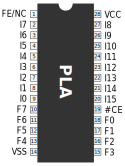
\includegraphics[width=\myupto{5cm}]{pinout}
    \caption{PLA pinout}
    \label{fig:pinout}
\end{figure}

\section{Electrical Properties}

In this section the results of measurements of some electrical properties of
original PLAs and different PLA replacements are shown. Their meaning for
the inner workings of the C64 is discussed.

\subsection{Devices Under Test}

The measurements for this document were done with one sample of each of the
two most frequently used bipolar PLAs, the Signetics 82S100 and the
Fairchild 93459PC. Three samples of the 906114-01 with different date codes
were also tested. Finally three PLA replacements were checked, the EPROM
STMicroelectronics M27C512-90B6, which is said to be the EPROM ideally
suited for this usage, the SuperPLA V2\footnote{While this document has been
written, Super PLA V3 has been released, it can replace PLAs of multiple
Commodore devices} from Individual Computers and the realPLA, which is
introduced in this document.

Gerrit Heitsch found another PLA type in a C64 which seems to be
manufactured by Fujitsu, according to its package shape and printing. This
type has a much lower power consumption than other original PLAs. It was not
examined for this document yet, but listed for the sake of completeness.

Table \ref{tab:dut} lists all devices under test (DUTs). This table contains
also the voltage of an output high level $\myVOH$. This is a valuable
indicator to the semiconductor technology used. However, the technology is
listed in the datasheets for most of the parts.

As a rough guideline the bipolar parts have a $\myVOH$ of about
$\myVCC - \SI{1.0}{\volt}$. The NMOS parts have a $\myVOH$ of $\myVCC -
\SI{1.3}{\volt}$, where \SI{1.3}{\volt} is $\myVth$ of an N-channel FET used
in the pad buffer totem pole. Details about the actual circuitry used there
will be described in section \ref{sec:mos-plas-inner-working}. The CMOS parts
have a $\myVOH$ of about $\myVCC$. The SuperPLA is a special case, refer to
section \ref{sec:superpla-tech} for details.

\begin{table}
\begin{minipage}{\linewidth}
    \tabletextsize
    \centering
    \begin{tabularx}{\mywidthfull}{l|X|c|l}
        \toprule
        Package & Type & $V_{OH}$ & Technology \\
        Label   &      &    [V]   &            \\
        \midrule
        N82S100N S C64 K8303   & Signetics 82S100    & 4.2 & Bipolar \\
        93459 PC F 8235        & Fairchild 93459PC   & 3.9 & Bipolar \\
        906114-01 2683         & MOS 7700R1          & 3.7 & NMOS \\
        906114-01 4885         & MOS 8700R2          & 3.8 & NMOS \\
        906114-01 2488         & MOS 8700R2          & 3.7 & NMOS \\
        M27C512-90B6           & EPROM M27C512-90B6  & 4.9 & CMOS \\
        SuperPLA               & SuperPLA V2         & 4.0 & CMOS/NMOS\footnote{Refer to text for details}\\
        realPLA                & realPLA             & 5.0 & CMOS \\
        \bottomrule
    \end{tabularx}
    \caption{PLA devices under test}
    \label{tab:dut}
\end{minipage}
\end{table}

\subsection{Power Consumption}

One of the most impressive properties of the PLA is: It gets quite hot for
the little work it has to do. To get an impression about their static power
dissipation, the devices were mounted on a breadboard. \#OE was
connected to GND. All inputs were pulled high, the outputs did not have a load.
The current at $\myVCC$ was measured with a multimeter.

Additionally the temperature was captured with an infrared thermometer in
the middle of the chip package's surface at an ambient temperature of 24
$^\circ$C. Note that the temperature is a rough estimation only. In some
cases the temperature is higher for a part which needs less power compared
to another part. The reason may be different physical properties of the chip
package\footnote{All of them where plastic packages} or simply inaccurate
temperature measurements.

Table \ref{tab:plapwr} shows the results of these measurements.

The 82S100 and the 93459 use bipolar technology, basically TTL or Schottky
TTL. They have the highest power consumption.

Also the NMOS implementation has a quite high power dissipation, which is
caused by the depletion load NMOS logic which needs relatively strong pull-up
devices to get the same switching speed as the bipolar original.

The pure CMOS variants EPROM and realPLA have the lowest idle power consumption.

\label{sec:superpla-tech} The PLD used in the SuperPLA uses CMOS technology
according to its datasheet \cite{Mach110}. But the relatively high static
power consumption and its $\myVOH$ of only \SI{4.0}{\volt} (refer to table
\ref{tab:dut}) shows that it must use some kind of hybrid logic, e.g., pseudo
NMOS logic. This is indirectly confirmed by some figures in that datasheet,
e.g., the output driver uses an NMOS totem pole instead of a real CMOS totem
pole, most likely for higher speed vs. chip area compared with PMOS FETs.

\begin{table}
    \tabletextsize
    \centering
    \begin{tabularx}{\mywidthnarrow}{X|c|c}
        \toprule
        DUT & $I_\mathrm{idle} $ [\si{\milli\ampere}] & $T$ [\si{\celsius}]
        \\
        \midrule
        82S100            & 102 & 45 \\
        93459PC           &  98 & 57 \\
        7700R1 (2683)     &  92 & 52 \\
        8700R2 (4885)     &  90 & 53 \\
        8700R2 (2488)     &  86 & 39 \\
        M27C512-90B6      &   4 & 26 \\
        SuperPLA          &  68 & 42 \\
        realPLA           &  13 & 28 \\
        \bottomrule
    \end{tabularx}
    \caption{PLA power consumption and package temperature}
    \label{tab:plapwr}
\end{table}

\subsection{Propagation Delay}
\label{sec:propagation-delay}

The propagation delay of the PLA is very important for the correct work of
the C64. For example, the \#CASRAM signal must be delayed by the PLA by at
least a certain time. On the other hand, the propagation delay must not be
too large, otherwise e.g., setup times of the chips which get their select
signals too late may be violated.

The \#CAS signal from the VIC-II is also used to multiplex the address bus
for the DRAM address inputs. This is done with U13 and U25 (74LS257), which
have a maximum propagation delay from their select input (\#CASRAM) to their
outputs of \SI{24}{\nano\second} \cite{TI257}. Typical DRAM chips used in
the C64 have an address setup time of at least \SI{0}{\nano\second} before
\#CAS, an example is the HM4864A (\cite{Hita4846}). This means that the
\#CASRAM signal must be delayed by at least this time, otherwise the DRAMs
would latch the wrong column address. This timing dependency could be called
a design flaw in the C64. Figure \ref{fig:casram-race} shows that the
multiplexed address changes about \SI{15}{\nano\second} after \#CAS and
becomes stable just about \SI{10}{\nano\second} before \#CASRAM gets active on
this board.

\begin{figure}
    \centering
    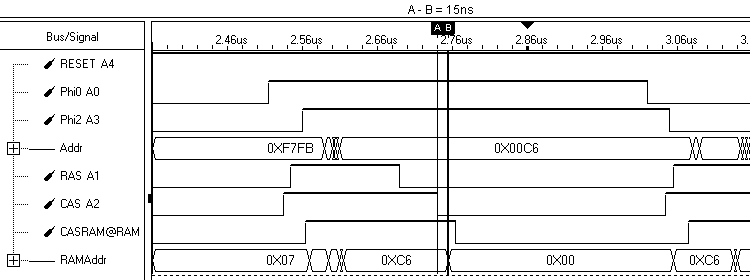
\includegraphics[width=\myupto{14cm}]{CASRAM-timing-bw}
    \caption{The \#CAS race}
    \label{fig:casram-race}
\end{figure}

The measurements shown here were done with a 200 MHz logic analyzer, so the
error is about $\pm \SI{5}{\nano\second}$. The input signals \#CAS and \#GAME
were connected to a binary counter. The output signals were sampled with a
threshold voltage of \SI{1.3}{\volt}, which is close to the threshold
voltage of NMOS inputs. \#CASRAM and \#ROMH have been chosen as outputs
because one of them has an inverted logic compared to the other one. This
may cause these two to have different delays. Figure \ref{fig:timing} shows
the output of one of these measurements. Table \ref{tab:pladelay} lists the
results. There may be sightly different propagation delays for situations
where several inputs change simultaneously, this has not been considered for
the measurements.

The propagation delays of original PLAs are of the order of
$\SI{25}{\nano\second} \pm \SI{5}{\nano\second}$. Note that the 7700R1 is
about \SI{5}{\nano\second} to \SI{10}{\nano\second} slower then the other
types. The bipolar PLAs have a slightly slower effective delay for low to
high transitions because their rising edges are very slow.

The EPROM M27C512-90B6 is a bit quicker than the original PLAs, but
still in the same ballpark.

The SuperPLA has its CASRAM delay tuned to be in the right order, which is
important for the DRAM control in the C64. But the delay of the other
outputs is much lower than the values seen on original parts. This seems not
to play a role usually, but there may be C64 boards and cartridges which may
have problems with this difference. Note that the logic in the SuperPLA
inhibits that other outputs to become low when \#CASRAM is still low, which
would lead to overlapping chip selects otherwise, due do the different delays.

The realPLA was designed to have an authentic delay and to have matched
delays among all outputs. This measurement confirmed that this aim was reached.

\begin{figure}
    \centering
    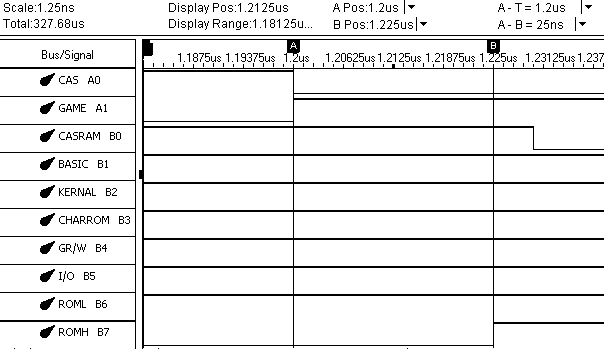
\includegraphics[width=\myupto{12cm}]{timing-bw}
    \caption{Example propagation delay measurement, DUT is 8700R2 (2488)}
    \label{fig:timing}
\end{figure}

\begin{table}
    \tabletextsize
    \centering
    \begin{tabularx}{\mywidthwide}{X|c|c|c|c}
        \toprule
            & \multicolumn{2}{c|}{\#CASRAM} & \multicolumn{2}{c}{\#ROMH} \\
        DUT & $T_{pdLH}$ & $T_{pdHL}$ & $T_{pdLH}$ & $T_{pdHL}$ \\
        \midrule
        82S100            & 35 & 25 & 25 & 25 \\
        93459PC           & 35 & 20 & 35 & 20 \\
        7700R1 (2683)     & 30 & 35 & 40 & 30 \\
        8700R2 (4885)     & 30 & 25 & 25 & 30 \\
        8700R2 (2488)     & 20 & 30 & 25 & 25 \\
        M27C512-90B6      & 20 & 20 & 20 & 20 \\
        SuperPLA          & 25 & 30 & 10 & 10 \\
        realPLA           & 25 & 30 & 25 & 30 \\
        \bottomrule
    \end{tabularx}
    \caption{Propagation delays [ns]}
    \label{tab:pladelay}
\end{table}


\subsection{Slew Rate}
\label{sec:slew-rate}

Some of the signals generated by the PLA are connected to long PCB traces
and connected to the Expansion Port, which may be connected using a ribbon
cable (as in the SX64) or may have a port expander or large PCB attached to
it. Signals with very steep edges could cause undesirable effects because of
reflections on the PCB traces or result in strong switching noise.

To get an impression of the slew rate of all PLAs tested, they were
connected to a test circuit. One of the inputs of each PLA was connected to
a clock signal, one of the outputs was loaded with a capacitor (82 pF, which is
a quite heavy load already) and captured with a digital scope. The scope I was
using had a sample rate of 100 Msamples/s only, so the slew rates are a rough
guess only.

A noticeable result of this measurement series is that bipolar and NMOS/CMOS
PLAs have very different slew rates. The falling edge and the rising edge of
the NMOS and CMOS PLAs are nearly symmetric, at least in the range between 1
V and 3 V.

However, the voltage of the bipolar PLAs raises very slowly over the whole
voltage range but drops quite quickly. The reason is most likely an output
stage similar to what is used in LS-TTL.

\begin{figure}
    \begin{minipage}{0.45\linewidth}
        \centering
        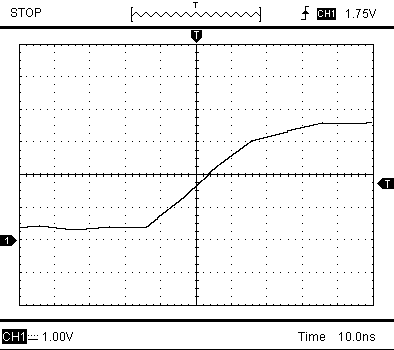
\includegraphics[width=\textwidth]{82s100-rise}
        \caption{82S100 - rising edge}
        \label{fig:82S100-rise}
    \end{minipage}
    \hfill
    \begin{minipage}{0.45\linewidth}
        \centering
        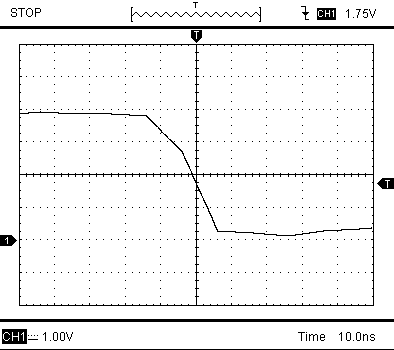
\includegraphics[width=\textwidth]{82s100-fall}
        \caption{82S100 - falling edge}
        \label{fig:82S100-fall}
    \end{minipage}
\end{figure}

\begin{figure}
    \begin{minipage}{0.45\linewidth}
        \centering
        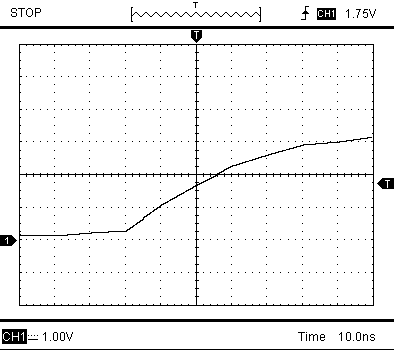
\includegraphics[width=\textwidth]{8235-rise}
        \caption{93459PC - rising edge}
        \label{fig:93459PC-rise}
    \end{minipage}
    \hfill
    \begin{minipage}{0.45\linewidth}
        \centering
        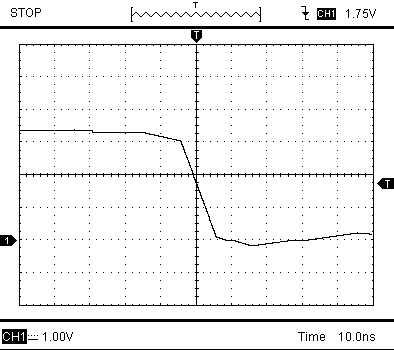
\includegraphics[width=\textwidth]{8235-fall}
        \caption{93459PC - falling edge}
        \label{fig:93459PC-fall}
    \end{minipage}
\end{figure}

\begin{figure}
    \begin{minipage}{0.45\linewidth}
        \centering
        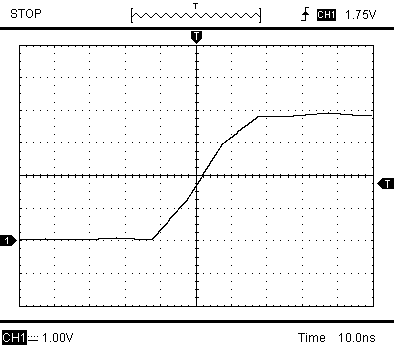
\includegraphics[width=\textwidth]{2683-rise}
        \caption{7700R1 (2683) - rising edge}
        \label{fig:7700R1-2683-rise}
    \end{minipage}
    \hfill
    \begin{minipage}{0.45\linewidth}
        \centering
        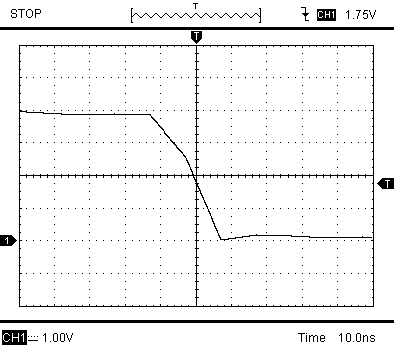
\includegraphics[width=\textwidth]{2683-fall}
        \caption{7700R1 (2683) - falling edge}
        \label{fig:7700R1-2683-fall}
    \end{minipage}
\end{figure}

\begin{figure}
    \begin{minipage}{0.45\linewidth}
        \centering
        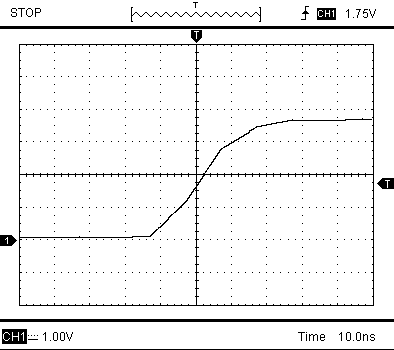
\includegraphics[width=\textwidth]{4885-rise}
        \caption{8700R2 (4885) - rising edge}
        \label{fig:8700R2-4885-rise}
    \end{minipage}
    \hfill
    \begin{minipage}{0.45\linewidth}
        \centering
        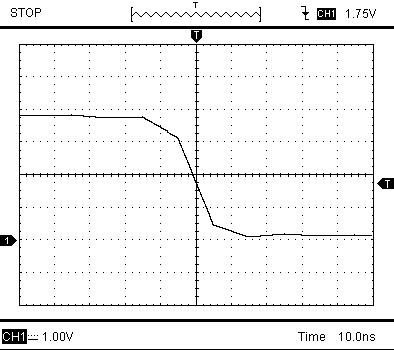
\includegraphics[width=\textwidth]{4885-fall}
        \caption{8700R2 (4885) - falling edge}
        \label{fig:8700R2-4885-fall}
    \end{minipage}
\end{figure}

\begin{figure}
    \begin{minipage}{0.45\linewidth}
        \centering
        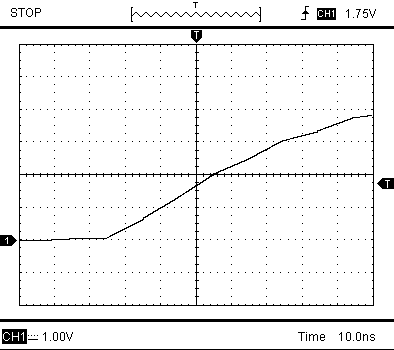
\includegraphics[width=\textwidth]{eprom-rise}
        \caption{M27C512-90B6 - rising edge}
        \label{fig:eprom-rise}
    \end{minipage}
    \hfill
    \begin{minipage}{0.45\linewidth}
        \centering
        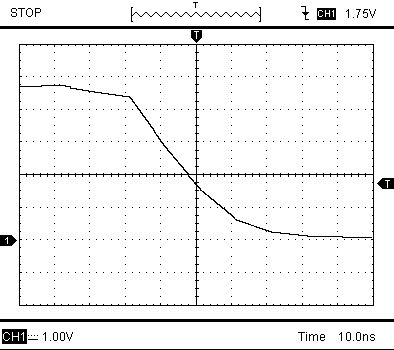
\includegraphics[width=\textwidth]{eprom-fall}
        \caption{M27C512-90B6 - falling edge}
        \label{fig:eprom-fall}
    \end{minipage}
\end{figure}

\begin{figure}
    \begin{minipage}{0.45\linewidth}
        \centering
        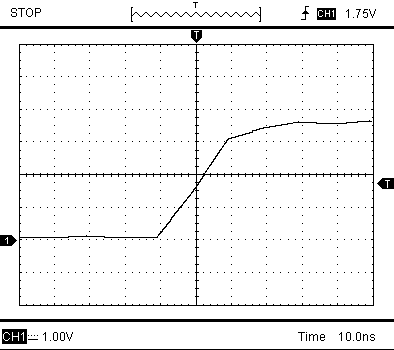
\includegraphics[width=\textwidth]{superpla-rise}
        \caption{SuperPLA - rising edge}
        \label{fig:superpla-rise}
    \end{minipage}
    \hfill
    \begin{minipage}{0.45\linewidth}
        \centering
        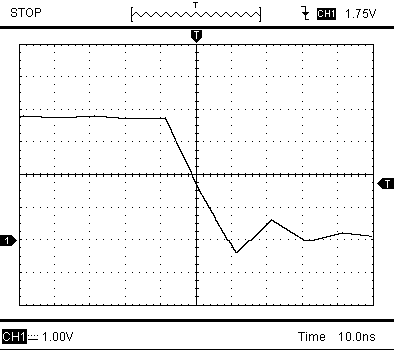
\includegraphics[width=\textwidth]{superpla-fall}
        \caption{SuperPLA - falling edge}
        \label{fig:superpla-fall}
    \end{minipage}
\end{figure}

\begin{figure}
    \begin{minipage}{0.45\linewidth}
        \centering
        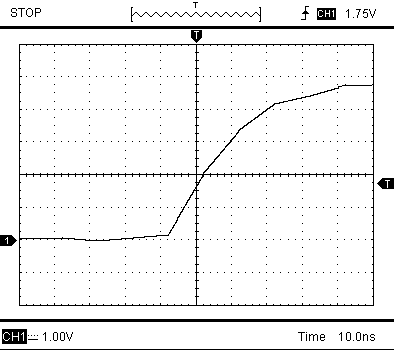
\includegraphics[width=\textwidth]{realpla-rise}
        \caption{realPLA - rising edge}
        \label{fig:realpla-rise}
    \end{minipage}
    \hfill
    \begin{minipage}{0.45\linewidth}
        \centering
        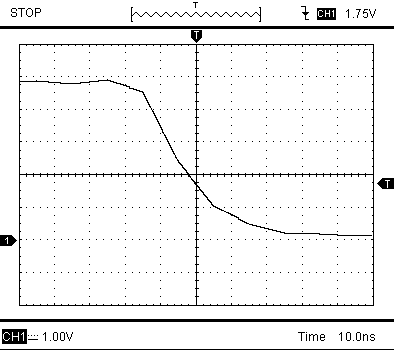
\includegraphics[width=\textwidth]{realpla-fall}
        \caption{realPLA - falling edge}
        \label{fig:realpla-fall}
    \end{minipage}
\end{figure}
%\afterpage{\clearpage}

\subsection{Overlapping Chip Selects}

A potential problem with PLAs and PLA replacements is that they could
activate multiple chip select signals at the same time. A reason for that
can be slower high to low transition times than low to high or different
propagation delays for different signal paths. Temporary bus contentions
caused by these effects could lead to higher power dissipation and therefore
higher heat generation in the chips involved.

After some investigations regarding this topic at \cite{esl11}, François
Léveillé had the idea to measure the power consumption of a C64 with
different PLAs attached. He did not elaborate this interesting experiment
very much, so it was repeated for this document.

Two different C64s of revision 250407 were used. The 5V rail was cut at
inductor L5 and the current was measured there. The supply current of such
a C64 at the 5V line is about 50 mA higher when the computer is at room
temperature than when it is warm. So in all cases the C64s have been left
running with the BASIC screen shown until the current consumption was stable.

In a second experiment the plain $\myVCC$ current of the PLA was measured at
the same state of the C64. This can be subtracted from the overall current
to calculate the power consumption of the rest of the C64.

Table \ref{tab:board-pwr} shows the result of these measurements, sorted by
board supply current at 5V without PLA supply current. Note that the first
board had the KERNAL ROM replaced with a CMOS type, which is the reason for its
lower overall power consumption.

\begin{table}
    \tabletextsize
    \centering
    \begin{tabularx}{\mywidthwide}{X|c|c|c}
        \toprule
        DUT & Overall  & PLA      & Board w/o PLA \\
            & $I$ [\si{\milli\ampere}] & $I$ [\si{\milli\ampere}] & $I$ [\si{\milli\ampere}] \\
        \midrule
        SuperPLA      &     695 &  59 &         636 \\
        8700R2 (2488) &     720 &  82 &         638 \\
        8700R2 (4885) &     721 &  82 &         639 \\
        M27C512-90B6  &     647 &   6 &         641 \\
        93459PC       &     736 &  86 &         650 \\
        \midrule
        \multicolumn{4}{l}{Different Board, different PLAs:} \\
        \midrule
        realPLA       &     782 &  15 &         767 \\
        M27C512-90B6  &     775 &   6 &         769 \\
        SuperPLA      &     837 &  68 &         769 \\
        82S100        &     875 & 105 &         770 \\
        \bottomrule
    \end{tabularx}
    \caption{Board power consumption depending from PLA}
    \label{tab:board-pwr}
\end{table}


The results show that the current differs, in addition to the different power
consumptions of the PLAs themselves. The 93459PC causes the rest of the C64
to draw about 10 mA more, which confirms the theory by François Léveillé.

However, the additional 10 mA compared with the overall 800 mA are a bit
more then 1\%, distributed over at least two chips. This will not cause
a noticeably increased heat generation nor reduced life time.

A closer look at the propagation delays and slew rates shown in section \ref
{sec:slew-rate} reveals that the Fairchild 93459PC has very quick falling
edges and very slow rising edges. This may lead to a bus contention with a
duration of about \SI{15}{\nano\second} per transistion, which explains the
slightly higher current.

\chapter{The Inner Workings of a CSG PLA}
\label{sec:mos-plas-inner-working}

To investigate the actual implementation of the PLA in the part which was
used most often in C64s, the MOS 7700R2/8700R1, they have been decapped and
photographed under a microscope for this document.

To get rid off the package, the PLAs have been cooked in rosin two times for
several hours. The abietic acid contained in rosin dissolved the plastic
package. Finally the dies have been cleaned in isopropyl
alcohol. Figure \ref{fig:decap1} et seq. show this procedure.

With these die shots the masks of the 8700R1 have been redrawn. The resulting
chip layout was used to draw the schematics of the PLA.

\begin{figure}
    \centering
    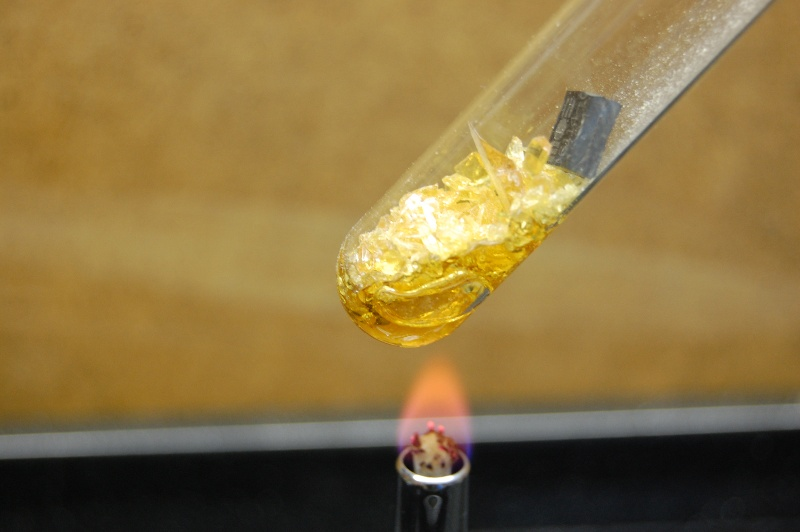
\includegraphics[width=\mywidthnarrow]{decap1}
    \caption{The decapping procedure starts}
    \label{fig:decap1}
\end{figure}
\begin{figure}
    \centering
    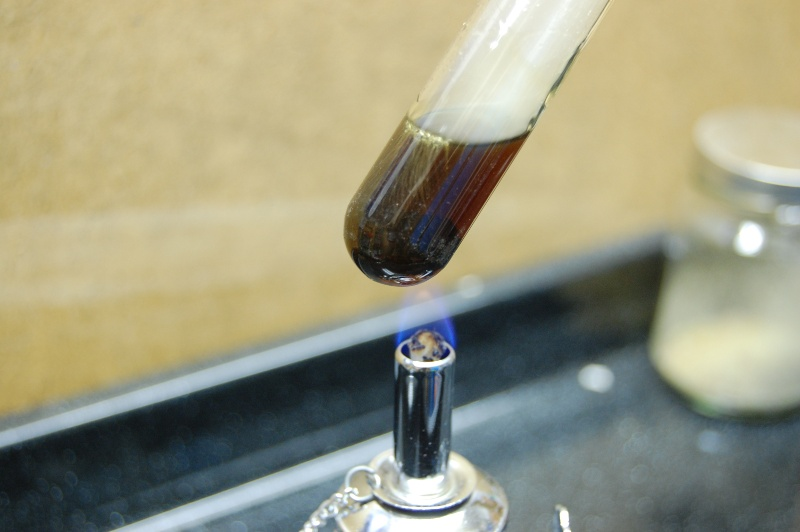
\includegraphics[width=\mywidthnarrow]{decap2}
    \caption{The package starts to dissolve}
    \label{fig:decap2}
\end{figure}
\begin{figure}
    \centering
    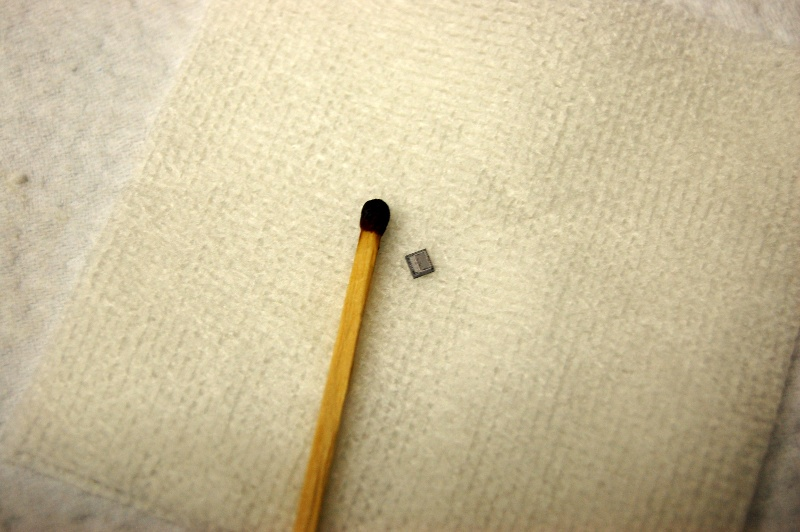
\includegraphics[width=\mywidthnarrow]{decap3}
    \caption{The die decapped and cleaned}
    \label{fig:decap3}
\end{figure}

\section{The Original Designers}

Even though the overall design of the PLA is not very complex, it may
have been challenging to build the NMOS part with the same speed as the
original bipolar part. It needs only approximately 25 ns for the whole row
of gates comprising an input super buffer, another super buffer, a NOR array
for the product term, another NOR array for the sum term, a super buffer and
the pad push-pull buffer. It was designed by Dave DiOrio, he recalls, ``It
was a rather simple chip select circuitry.''

The PLA was produced over many years, but not all replacements for third
party chips by Commodore had such a good fate. ``At one time there was a
shortage of some of the TTL components used on the platform so they even
tried replacing those chips with an NMOS `equivalent' that never really
panned out due to speed problems,'' recalls James Redfield.

The 7700R2 PLA has the initials ``RD'' and ``JB'' written on the metal
layer. JB is the mask designer Joan Brenneke. She drew the polygons most
likely, her colleague \textit{RD}\footnote {Name still unknown} digitized
the layout into the Calma CAD system finally. Figure \ref {fig:mos-initials}
shows their initials.

\begin{figure}
    \centering
    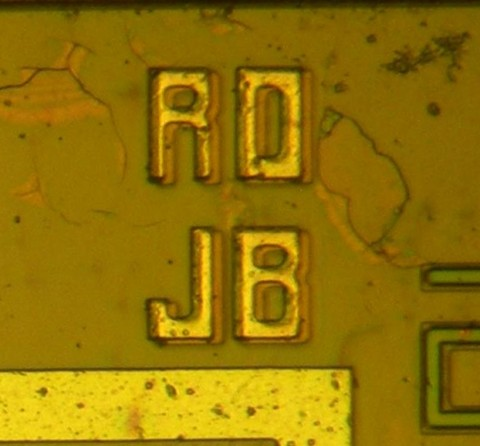
\includegraphics[width=\mywidthnarrow]{initials}
    \caption{Initials found on the PLA 7700R2}
    \label{fig:mos-initials}
\end{figure}

\section{NMOS Process Generations}

CSG evolved several generations of NMOS manufacturing. Before about 1983,
the chips were numbered with a 6xxx scheme. Their manufacturing process was
commonly referred to as NMOS and had a critical dimension (CD)          of
about\footnote{Measured on die shots} \SI{8}{\micro\meter} for the 6502,
over the years they seem to have been reduced, The VIC-II (MOS 6567) was
implemented with \SI{6}{\micro\meter} channel length\footnote{According
to James Redfield and Bret Raymis, this confirms measurements on die shots}.
The 7xxx chips appeared in about 1983. This process was called HMOS1. Only
one year later, the next generation called HMOS2 was in use already, which
was numbered 8xxx. The design rules had a CD                             of
\SI{5}{\micro\meter}\footnote{According to Bret Raymis}. The numbering
scheme was not used consistently in all cases, for example the CIA was still
called 6526(A) when it was manufactured using the HMOS2 process.

Dave DiOrio explains, ``These dimensions were `drawn' dimensions. Through
the fabrication process there would be etching and effects that provided a
different effective gate length.'' This may be the reason that the PLA die
shots look like they use a channel width of approximately \SI {4}{
\micro\meter}, although the nominal gate length were larger.

There is no official definition for HMOS1 and HMOS2. Dan Morris recalls
``All companies used similar naming conventions. [...] The photo process
sets the classical shrink sequence. As photo equipment improves, smaller
geometries can be resolved. Scaling through photo shrinkage allowed circuit
designs to be reused without the need to redesign them. A 20\% linear shrink
would run [approximately] 40\% faster at 40\% lower power. and reduce
production cost by 40\% as well. So process engineering's job was to develop
a 20\% shrink process about every 12 months. The number sequence identified
each shrink step (HMOS1 to HMOS2) that process was running. When a process
could no longer be shrunk a new process was developed and used the new
design rules as its starting point. (NMOS to HMOS)''

Figure \ref{fig:7700-8700-dies} shows the size of the two CSG PLAs. There is
a noticeable 10\% linear process shrink between these two revisions.
Unfortunately the surface of the 7700R2 got damaged when it was decapped.
Figure \ref{fig:7700-8700-shrink2} shows (more or less) that the channel
length was changed by the same factor, which confirms a photo shrink with
changes in the metal layer for the labels only. When putting a die shot of
the 7700R2 on top of a scaled die shot of the 8800R1, it can be seen that
the match very well.

With the term \textit{NMOS} this document refers to NMOS logic in general, no
matter which process or structure size was used to manufacture it.

\begin{figure}
    \centering
    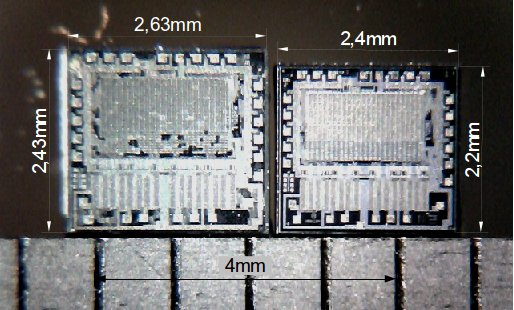
\includegraphics[width=\myupto{10cm}]{7700-8700-scale}
    \caption{Sizes of MOS 7700R2 and MOS 8700R1 compared}
    \label{fig:7700-8700-dies}
\end{figure}

\begin{figure}
    \centering
    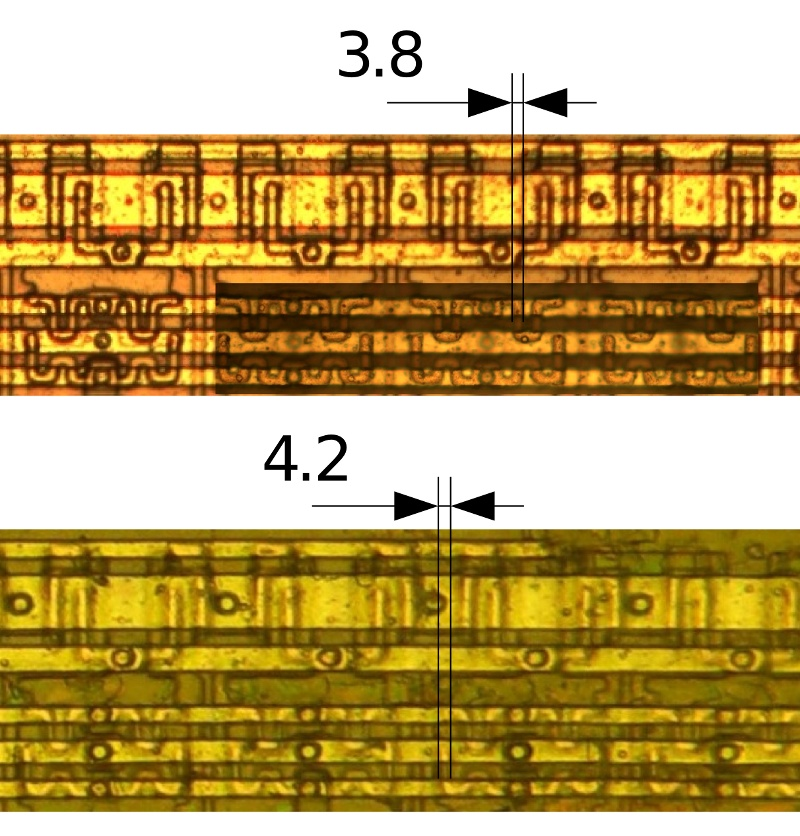
\includegraphics[width=\myupto{8cm}]{7700-8700-shrink2}
    \caption{Approximate channel length of 7700R1 and 8700R1}
    \label{fig:7700-8700-shrink2}
\end{figure}

\section{Reliability Failures}

People who repair Commodore computers notice that the early PLAs fail
quite often. Bil Herd recalls ``By far the worst chip failure mode we had
was the PLA around 1982-83 as it was suffering from poor passivation. It
would get the `purple creeping crud' which was corrosion under the
protective layer.''

Dan Morris knows the reason for this issue: ``The inter-layer glass
(Low Temp Oxide or LTO) is doped with Boron and Phosphorus atoms. Boron and
phosphorus are added to soften the glass and cause it to flow at lower
temperatures. The flow smooths the surface of the circuit dramatically
improving step coverage for the aluminum interconnections. Boron
concentrations above 4\% really accelerates the glass flow. Unfortunately
raising the Boron concentration above 4\% also sets up a strong but
relatively slow corrosion reaction with aluminum. This is a reliability time
bomb. As soon as the field failures demonstrated a problem. The process was
changed to reduce the Boron to less than 3\%. Unfortunately, many, many
computers shipped with this problem first.''

\begin{mytextframe}{.9\textwidth} \textbf{Dan Morris} managed the
manufacturing test and product engineering for the California semicondutor
facility\footnote{Frontier Semiconductors, acquired by Commodore} from
September 1981 to 1985. His first task was to set up a silicon gate CMOS
fab, this fab made metal gate CMOS up to then. ``About three months into our
production ramp up we got the word on a Friday night that we needed to stop
all work and immediately convert the fab to run the NMOS process from Valley
Forge. [...] The CMOS process we developed never went to production.''

``Our orders were `copy exactly', no deviations allowed. That was a tall
order, given different equipment and different process skills. We worked
without sleep for 5 days. We took each process step and duplicated it on
each piece of equipment and started the first fab lot on the 6th day. We
ramped the fab to full production 4 weeks later after the first lot proved
successful with yields better than the Valley Forge fab.'' The California
facility produced the majority of the integrated circuits for the VIC 20 and
Commodore 64 computers.

Dan Morris also developed low cost test systems for wafer and final test
of the audio and video chips.
\end{mytextframe}

The PLA seems to be more prone to failures than e.g., the 6510 or 8500 CPU.
This may be caused by the fact that it was among the first chips made with
the HMOS1 process. Another factor could be that it has a quite high power
dissipation on a small die area compared to other chips. Its high
temperature may speed up its aging, e.g., because of mechanical stress and
by speeding up processes like electromigration \cite{Hoffmann06}. Also the
7360 TED and the 7501 CPU are reported to fail quite often.

\section{Block Diagram}

Figure \ref{fig:pla-block-dia} shows the function blocks of the CSG PLA
and their approximate position on the die. These function blocks will be
described in the subsequent sections.

\begin{figure}
    \centering
    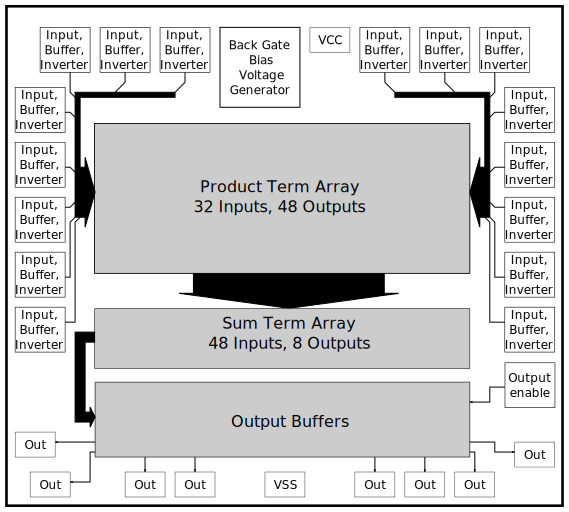
\includegraphics[width=\myupto{9cm}]{block-diagram}
    \caption{Block Diagram of the CSG PLA}
    \label{fig:pla-block-dia}
\end{figure}

\clearpage
\section{Input Stage}

All 16 function inputs of the PLA have the same input stage. An input
contains a basic ESD protection made of a grounded gate FET T1 (GGNMOS).
With a width of only \SI{50}{\micro\meter} this protection can only
stand small ESD stress \cite{Sem08}. The diffusion resistor R1 connects to the
input pad I0. This resistor additionally limits current peaks, which supports
the ESD protection mechanism.

The input signal is connected to a large inverting super buffer T2..T5 which
creates an inverted signal \#I0B. Additionally there are two inverting super
buffers T6..T9 and T10..T13 to create a buffered signal I0B. These two output
signals I0B and \#I0B are connected to the rows of the AND array.

Note that the depletion mode pull-up devices of the final stages, T4 and T12
are very strong drivers, their width to length ratio (W/L) is about 35/6.
They must be that strong to pull up all of the 48 small gates in the NOR
array quickly enough.

Figure \ref{fig:inputs-shot} shows a photo of an input stage, the redrawn
layout is shown in figure \ref{fig:inputs-layout} and the schematics in figure
\ref{fig:inputs-schem}.

\begin{figure}
    \centering
    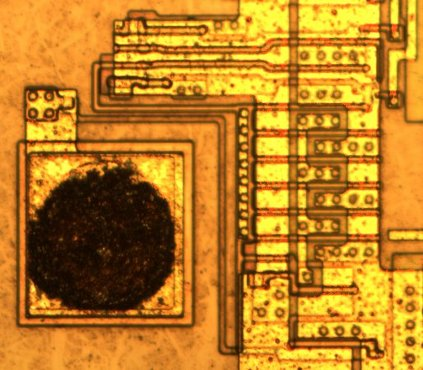
\includegraphics[width=\myupto{11cm}]{inputs-shot}
    \caption{Die photograph of ESD protection, input buffer and inverter}
    \label{fig:inputs-shot}
\end{figure}


\begin{figure}
    \centering
    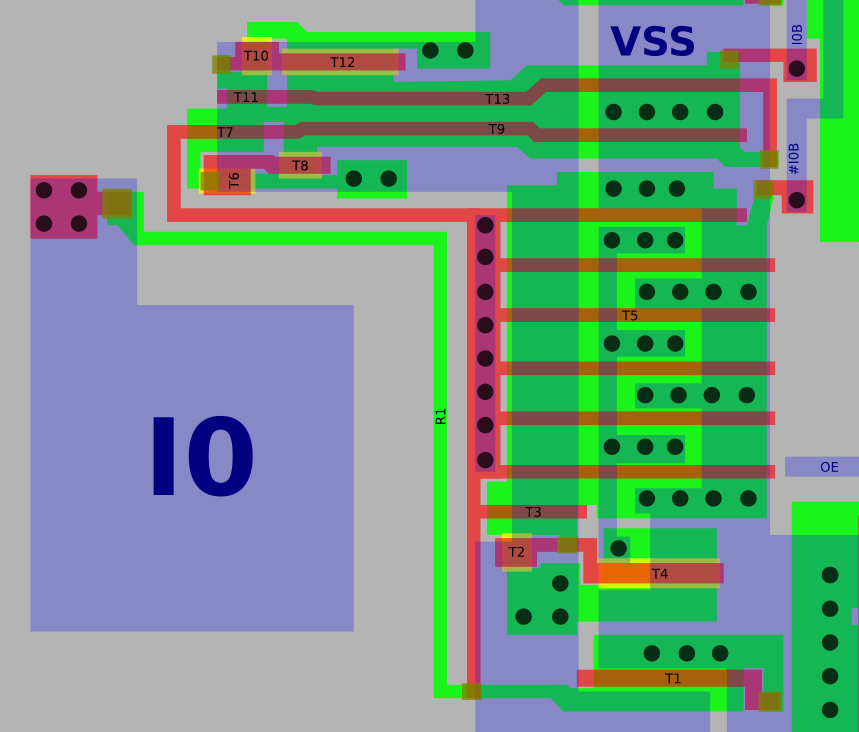
\includegraphics[width=\myupto{11cm}]{inputs-layout}
    \caption{Layout of ESD protection, input buffer and inverter}
    \label{fig:inputs-layout}
\end{figure}

\begin{figure}
    \centering
    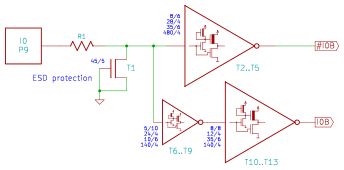
\includegraphics[width=\myupto{13cm}]{inputs-schem}
    \caption{Schematic of ESD protection, input buffer and inverter}
    \label{fig:inputs-schem}
\end{figure}

\clearpage
\section{Output Enable}

The output enable input contains the same ESD protection as the other inputs
(R17, T209). An inverting super buffer T210..T213 is used to prepare the
internal signal OE. Figures \ref{fig:oe-shot} to \ref{fig:oe-schem} show
a photograph, layout and schematics of this circuit.

\begin{figure}[htb]
    \centering
    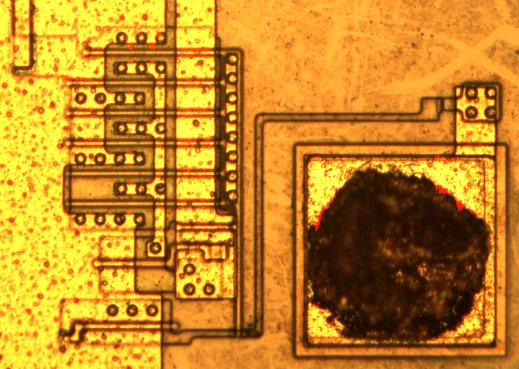
\includegraphics[width=\myupto{11.5cm}]{oe-shot}
    \caption{Die photograph of ESD protection and inverter for OE}
    \label{fig:oe-shot}
\end{figure}

\begin{figure}[htbp]
    \centering
    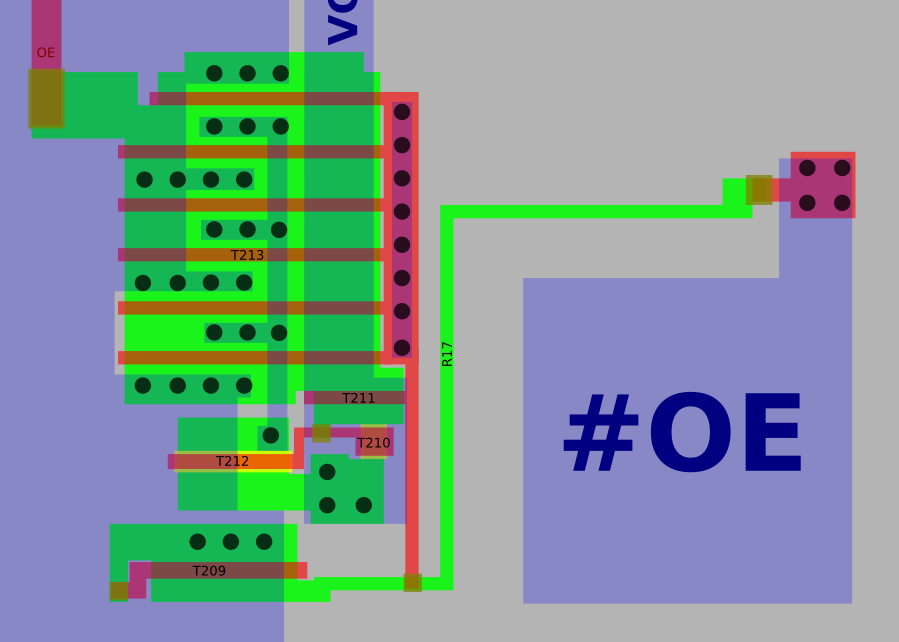
\includegraphics[width=\myupto{11.5cm}]{oe-layout}
    \caption{Layout of ESD protection and inverter for OE}
    \label{fig:oe-layout}
\end{figure}

\begin{figure}[htbp]
    \centering
    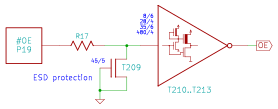
\includegraphics[width=\myupto{11cm}]{oe-schem}
    \caption{Schematic of ESD protection and inverter for OE}
    \label{fig:oe-schem}
\end{figure}

\clearpage
\section{Product Term Array}

A classical PLA contains a programmable AND array which has its outputs
connected to a programmable OR array \cite{Maini07}. The AND array is used for
product terms and the OR array for sum terms.

The actual implementation of the AND array is realized with NOR gates with
inverted inputs on the CSG PLAs, which has the same functionality according
to De Morgan's laws. This implementation is also explained in \cite{Mead79}.

The product term array has 32 inputs, I0B, \#I0B to I15B and \#I15B and 48
outputs P0 to P47. Each of these 48 output columns can carry the result
of a product term of the inputs.

Each input row is connected to 48 polysilicon tracks which can become gates
for enhancement mode FETs. The field oxide mask, which also defines the
diffusion layer, is used to program this array. Each of the 48 * 32 array
gates forms a FET only if it crosses a diffusion area. Otherwise it is just
a piece of non-functional polysilicon.

Each output column has a pull up circuit to pull it high when no FET in the
column is on. Any of the FETs in each column can pull the column down.
This circuit is used to implement NOR functions.

The die photograph and layout \ref{fig:product} show two inactive nodes in
the product term array and two nodes which were mask programmed to build
FETs. The same parts are also shown in the schematic \ref
{fig:product-schem}. To keep the numbering scheme simple, all gates have a
transistor annotation 'T...', although only some of them are real
transistors. The whole array is totally uniform, therefore only a part of it
is shown here.

Figure \ref{fig:pterms-visible} shows the encoding of the whole NOR array.
The product terms are nearly in the same order as it was extracted from an
82S100. The unused terms p8 and p29 were removed (refer to section
\ref{sec:pterms}) and replaced with the terms initially numbered p31 and
p30. So the numbering of the product terms is slightly different.

\begin{figure}[htbp]
    \centering
    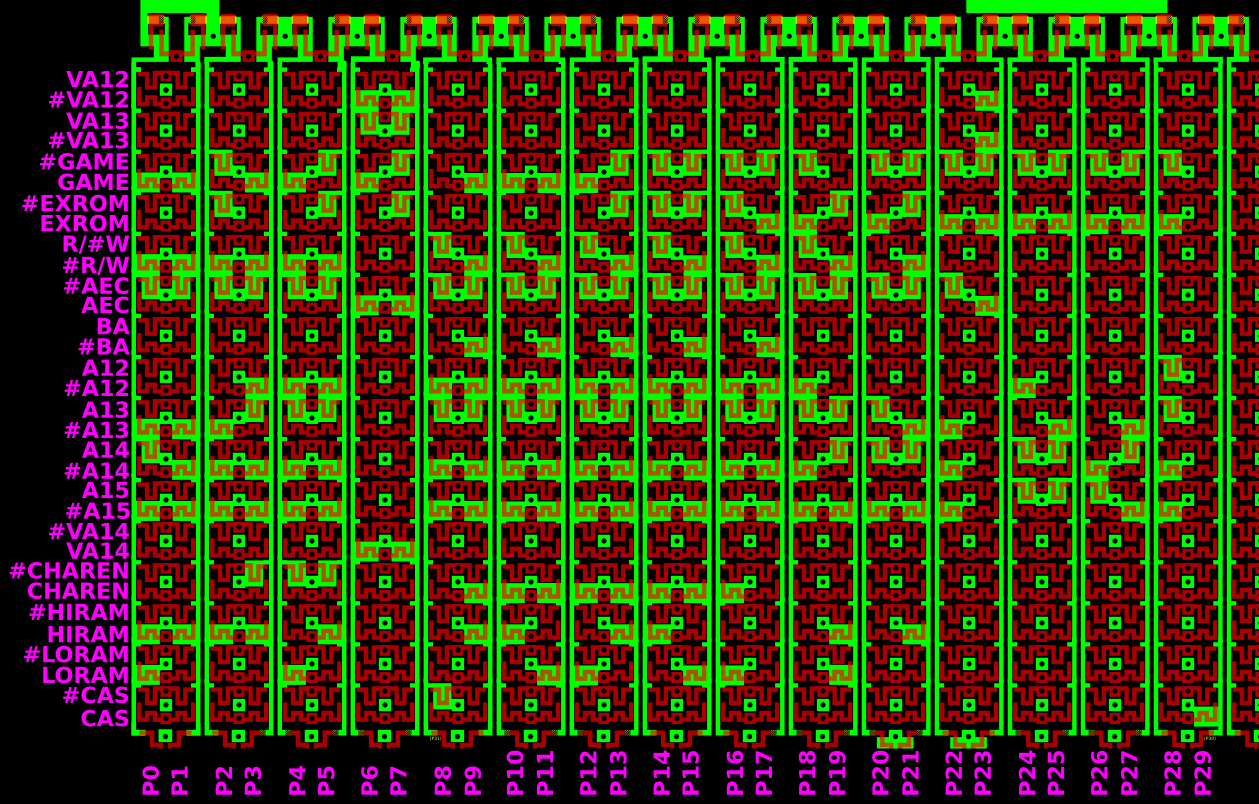
\includegraphics[width=\myupto{15cm}]{pterms-visible}
    \caption{Product terms made readable in the layout}
    \label{fig:pterms-visible}
\end{figure}

Figure \ref{fig:nor-shot-up} shows a high resolution detail of the pull-up
circuit, even the contact through gate oxide can be seen there. The two
images in figure \ref{fig:focal-planes} give a very good impression about
the third dimension of the chip's surface. The microscope was focused on the
active area at the first picture and on the poly or metal layer on the
second one.

\begin{figure}[htbp]
    \centering
    \subbottom[Die photograph]
    {
        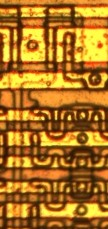
\includegraphics[height=6cm]{product-shot}
    }
    \subbottom[Layout]
    {
        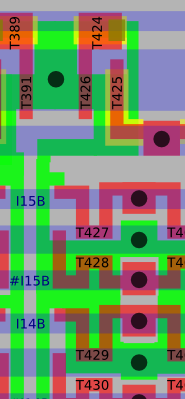
\includegraphics[height=6cm]{product-layout}
    }
    \caption{A part of the product term array}
    \label{fig:product}
\end{figure}

\begin{figure}[htbp]
    \centering
    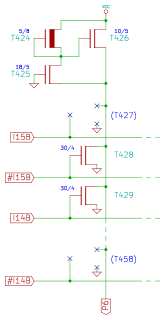
\includegraphics[width=6cm]{product-schem}
    \caption{Schematic of a part of the product term array}
    \label{fig:product-schem}
\end{figure}

\begin{figure}[htbp]
    \centering
    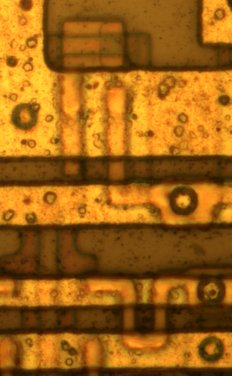
\includegraphics[width=5cm]{nor-shot-up}
    \caption{High resolution image of the pull-up part}
    \label{fig:nor-shot-up}
\end{figure}

\begin{figure}[htbp]
    \centering
    \subbottom[Focus on active area]
    {
        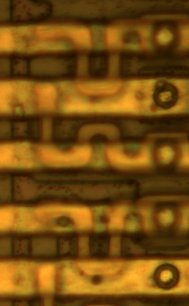
\includegraphics[width=3.5cm]{nor-shot1}
    }
    \subbottom[Focus on poly]
    {
        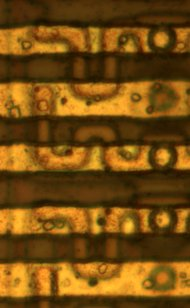
\includegraphics[width=3.5cm]{nor-shot2}
    }
    \caption{Different focal planes}
    \label{fig:focal-planes}
\end{figure}

The graphics also show the pull up circuit mentioned before. Because of its
relatively large width the pull up FET T426 is not a depletion mode FET but
an enhancement mode device. Its gate is pulled up to $\myVCC$ with the
depletion mode FET T424. This causes T426 to be switched on steadily.

The function of T425 could not be clarified. Its gate is tied to $\myVSS$,
therefore this FET is always off. One potential use of it could be
bootstrapping. In this case the parasitic capacity $C_{DS}$ of T425 would
pull down or push up the gate voltage of T426 for a short moment, whenever
the source voltage of this FET changes. This would increase its channel
resistance on falling edges and decrease it on rising edges. Note that the
drain-gate capacitance $C_{DG}$ even has an opposite effect. SPICE
simulations\footnote {MOSFET model level 3, various parasitic parameters
defined with generic values, L, W, AS, AD, PS, PD measured and entered} did
not reveal a useful effect of this transistor. Also simulations with a
zero-threshold device did not help. However, when a poly cap of a similar
size, e.g., $\SI{20}{\micro\meter} \times \SI{10}{\micro\meter}$ is put into
the simulation, there is a much stronger bootstrap effect, which speeds up
this gate by about \SI{1}{\nano\second}. Possibly the SPICE model
parameters were not chosen correctly to simulate the intended effect. So it
looks like the real reason for T425 is still unknown.

\begin{mytextframe}{.9\textwidth}
\textbf{The enhancement mode FET threshold voltage} $\myVth$ in the CSG chips
cannot be measured directly. However, it can be found by looking at the
output pad buffers: They are implemented using a totem pole made of two NMOS
FETs. When an output delivers a high level, the pull-up FET gets its gate
voltage from a super buffer with a depletion mode pull-up, which delivers
$\myVCC$ virtually. This NMOS pull-up can pull the output not higher than about
$\myVCC - \myVth$. Measurements showed that the output voltage is about
\SI{3.7}{\volt} to \SI{3.8}{\volt}, which means that $\myVth$ is
approximately \SI{1.3}{\volt}.


Note that $\myVth$ can not be measured on an input pad accurately, because
the inputs are connected to a super buffer with depletion mode devices in its
pull-up branches. A high level is only detected if the input voltage is
higher than the inverter voltage $\myVinv$, which is determined by the FET
size ratios. However, given the large ratios seen on CSG chips, $\myVinv$ is
not much higher than $\myVth$.
\end{mytextframe}

Unfortunately it is not possible to accurately simulate or calculate the dynamic
behaviour of these chips, because too few parameters are known.
However, some things can be calculated, for example the output
voltage of a product term $\myVO$. It depends on how many pull-down FETs are
switched on, the size of the FETs involved, $\myVCC$ and $\myVth$.

As an example $\myVO$ for a single pull-down device being active is calculated
here. The gate and source of a pull-up FET (e.g. T426) are at approximately
$\myVCC$ (\SI{5}{\volt}). Its source is at output voltage $\myVO$.
\begin{equation}
\label{eq:VGSu}     \myVGSu = \myVDSu = \myVCC - \myVO
\end{equation}
The drain of a pull-down FET (e.g. T428) is also at $\myVO$, its gate is at
$\myVCC$, due to the depletion mode super buffers, and the source at $\myVSS$
(\SI{0}{\volt}).
\begin{align}
\label{eq:VGSd}     \myVGSd &= \myVCC \\
\label{eq:VDSd}     \myVDSd &= \myVO
\end{align}
The ratio between pull-up device and pull-down device will be called $z$:
\begin{equation}
\label{eq:z}        z = \frac {\frac{W_d}{L_d}} {\frac{W_u}{L_u}}
\end{equation}

Because of (\ref{eq:VGSu}) $V_{GS} < V_{DS} + \myVth$ is valid,
the pull-up FET is saturated. So its drain current is calculated as follows:
\begin{equation}
\label{eq:sat}
    I = K \frac{W}{L} (V_{GS} - \myVth)^2
\end{equation}

With $K$ being a constant which describes some physical properties of the
FETs. Refer to \cite{Ray08} for details about $K$, (\ref{eq:sat}) and
(\ref{eq:nonsat}).

Because the pull-up device is a depletion mode FET, it is known that
$\myVO < \myVCC - \myVth$, which means that $V_{GS} > V_{DS} + \myVth$.
Therefore the pull-down FET is not saturated. For this case (\ref{eq:nonsat})
is used.
\begin{equation}
\label{eq:nonsat}
I = K \frac{W}{L} [ 2 (V_{GS} - \myVth) V_{DS} - V_{DS}^2 ]
\end{equation}
This equation can be written in a form which will be more handy later, the
result is (\ref{eq:nonsat2})\footnote{Thanks to Segher Boessenkool for pointing
me to the transformed equation. However, deriving it from the equation found
in most books needs a bit of magic.}.
\tabletextsize
\begin{align}
I &= K \frac{W}{L} [ 2 (V_{GS} - \myVth) V_{DS} - V_{DS}^2 ] \notag \\
  &= K \frac{W}{L} [ 2 V_{GS} V_{DS} - 2 V_{DS} \myVth - V_{DS}^2 ] \notag \\
  &= K \frac{W}{L} [ V_{GS}^2 - 2 V_{GS} \myVth + \myVth^2 \notag \\
  &    \qquad \qquad - V_{GS}^2 - V_{DS}^2 - \myVth^{2} + 2 V_{GS} V_{DS}
        \mymathbreak + 2 V_{GS} \myVth - 2 V_{DS} \myVth ] \notag \\
\label{eq:nonsat2}
  &= K \frac{W}{L} [ (V_{GS} - \myVth)^2 - (V_{GS} - V_{DS} - \myVth)^2 ]
\end{align}
\normalsize
The current flows through both FETs and there is no significant load current
once the circuit reached a static state, therefore (\ref{eq:sat}) and
(\ref{eq:nonsat2}) can be used:
\tabletextsize
\begin{align*}
    I_\mathrm{Du} &= I_\mathrm{Dd} \\
    K \frac{Wu}{Lu} (\myVGSu - \myVth)^2 &=
                    K \frac{Wd}{Ld} [ (\myVGSd - \myVth)^2
                    \mymathbreak - (\myVGSd - \myVDSd - \myVth)^2 ] \\
\end{align*}
\normalsize
With the values from (\ref{eq:VGSu}) to (\ref{eq:VDSd}):
\tabletextsize
\begin{align*}
    (\myVCC - \myVO - \myVth)^2 &=
                    z [ (\myVCC - \myVth)^2 - (\myVCC - \myVO - \myVth)^2 ] \\
    (\myVCC - \myVO - \myVth)^2 &=
                    z (\myVCC - \myVth)^2 - z (\myVCC - \myVO - \myVth)^2 \\
    (z+1) (\myVCC - \myVO - \myVth)^2 &=
                    z (\myVCC - \myVth)^2
\end{align*}
\normalsize

Both sides are positive:
\tabletextsize
\begin{align}
    \sqrt{z+1} (\myVCC - \myVO - \myVth) &=
                    \sqrt{z} (\myVCC - \myVth)                  \notag \\
    \sqrt{z+1} (\myVCC - \myVth) - \sqrt{z+1} \myVO &=
                    \sqrt{z} (\myVCC - \myVth)                  \notag \\
    (\sqrt{z+1} - \sqrt{z}) (\myVCC - \myVth) &= \sqrt{z+1} \myVO
                                                                \notag \\
    \myVO &= \frac{\sqrt{z+1} - \sqrt{z}}{\sqrt{z+1}} (\myVCC - \myVth)
                                                                \notag \\
\label{eq:vout}
    \myVO &= (1 - \frac{\sqrt{z}}{\sqrt{z+1}}) (\myVCC - \myVth)
\end{align}
\normalsize

Die shots show that $\frac{W_d}{L_d}$ is about $3 \frac{W_u}{L_u}$, so $z = 3$.
With $\myVCC = \SI{5}{V}$ to and $\myVth = \SI{1.3}{V}$ this results in:
\tabletextsize
\begin{align*}
    \myVO &= (1 - \frac{\sqrt{3}}{\sqrt{3+1}}) (\SI{5}{V} - \SI{1.3}{V}) \\
          &\sim \SI{0.5}{\volt}
\end{align*}
\normalsize

This gives a nice low level output. The voltage will be lower with more
pull-down FETs turned on, which is equivalent with higher values for $z$.

\begin{mytextframe}{.9\textwidth} \textbf{James Redfield} was hired
by Al Charpentier specifically to work on the VIC-II chip. Al Charpentier,
James Redfield and Dave DiOrio developed the VIC-II together. I asked James
about the methodology taken to develop the design of the Commodore chips.
``There were no logic simulations in those days,'' he explains, ``everything
was manual expect for pure transistor simulations with SPICE [...].''
% and except for the layout design
A custom chip design is a very complex work. To
give an impression of some of the steps needed to be done, James explains,
``Before joining Commodore, one of the grad courses I had taken was a class
in VLSI systems design.  That class used a book that was the authority for
NMOS circuit design at the time: `Introduction to VLSI Systems' by Carver
Mead and Lynn Conway \cite{Mead79}.  I would highly recommend that any
serious student of early VLSI design methodology purchase a copy of this
book if at all possible! [...] For example, chapter 1 walks the student
through calculations necessary to derive the proper transistor dimensions
that will establish logic switching thresholds that yield the greatest noise
immunity.  The inverter is the most basic element, it is analyzed to develop
the optimal aspect ratio (the optimal NMOS switching device W/L dimensions
to depletion device W/L dimensions).  Once established this ratio can easily
be extended to cover [other] logic elements. This optimal aspect ratio is
always the same for any given process technology.  Once it's been derived
the main consideration for sizing transistors is the load seen by each
gate.  To assist in sizing the transistors, my methodology was as follows.
At the start of the project I would run a series of simulations to generate
a table of load versus gate size delay information.  The circuit in the
simulation was a string of six inverters, each inverter connected to
identical load capacitance and the sizes on each inverter all set the same.
I would measure the delay time between nodes 3 and 5 in the inverter string
and divide by two (to average out rise versus fall delay).  I would then
have a table of delay versus transistor size for a wide range of load
capacitance that I would reference to size paths in the chip I was
building.  In logic devices, required timing for each path is dictated by
the frequency of the clock used to clock the launching and sampling
flip-flops.  The period of the clock divided by the number of logic gates
between each set of flops specified how fast each gate in the path needed to
be.  I would start with the sampling flop, estimate the input load of the
flop and select the size for gate driving the input based on that load and
the time budgeted for each gate in that path.  That gate having been sized I
could move back to the next gate and size that one.  This provided a
preliminary design that could then be simulated with spice [...].

Of course this is very simplified overview of the design process.  Many
factors could dictate other size choices for example die real-estate
available and power requirement are two other considerations.''
\end{mytextframe}

\clearpage
\section{Sum Term Array}

The sum terms are also implemented using a NOR array. The output signals are
inverted compared with a plain OR array, but this does not matter since the
final output will still go through amplifiers and can be programmed to be
inverted anyway.

Each output signal from the product term array is connected to a column of
polysilicon. Eight metal rows cross these columns. These rows carry the sum
terms \#F0 to \#F7. Each row has a pull-up circuit of the same kind as used in
the product term array.

The field oxide mask is used to program FETs, like in the other array.
Additionally contacts to metal are needed here. Obviously these contacts
are not at every potential FET, but only at FETs actually implemented. This
means that two masks had to be changed to program a PLA.

The ratio between pull-up FET and pull-down FETs is the same as in the
product term array.

Figures \ref{fig:sum-shot} to \ref{fig:sum-schem} show a photograph, layout
and schematics of this circuit.


\begin{figure}
    \centering
    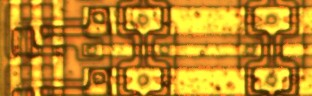
\includegraphics[width=\myupto{8cm}]{sum-shot}
    \caption{Die photograph of a part of the sum term array}
    \label{fig:sum-shot}
\end{figure}

\begin{figure}
    \centering
    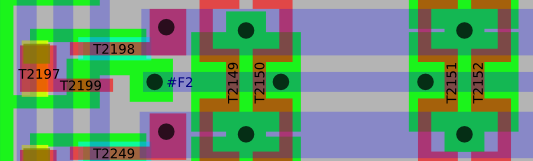
\includegraphics[width=\myupto{8cm}]{sum-layout}
    \caption{Layout of a part of the sum term array}
    \label{fig:sum-layout}
\end{figure}

\begin{figure}
    \centering
    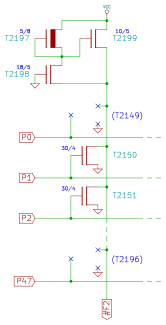
\includegraphics[width=\myupto{6cm}]{sum-schem}
    \caption{Schematic of a part of the sum term array}
    \label{fig:sum-schem}
\end{figure}


\clearpage
\section{Output Stage}

Each function result like \#F0 is inverted with a quick inverting super
buffer (T2302..T2305), which results in the complementary value F0. F0 and
\#F0 are combined with OE with a logical NAND function (T2306..T2310). The
resulting intermediate signals are buffered with two larger super buffers to
be able to drive the gates of the pad buffer quickly.

The push-pull totem poles for the output pads are really huge. These 16 FETs
take about 25\% of the chip area. Björn `JMP\$FCE2' Wieck examined their
drive strength. When an output is low, it can sink more than 80 mA while
still being in the linear region\footnote{Don't try this at home, the PLA
won't survive this for long}, i.e. the output is still below \SI{1.3}{\volt
} in this situation. When the output switched from low to high, the pull-up
FET will deliver the same current as long as the source voltage is still
very low, so also low to high transitions rise over the threshold voltage
quickly. Due to the characteristics of an N-channel FET the drive strength
decreases at higher output levels which result in lower $\myVGS$.

Figure \ref{fig:output-shot} to \ref{fig:output-schem} show photo, layout and
schematic diagram of the output stage.

\begin{figure}
    \centering
    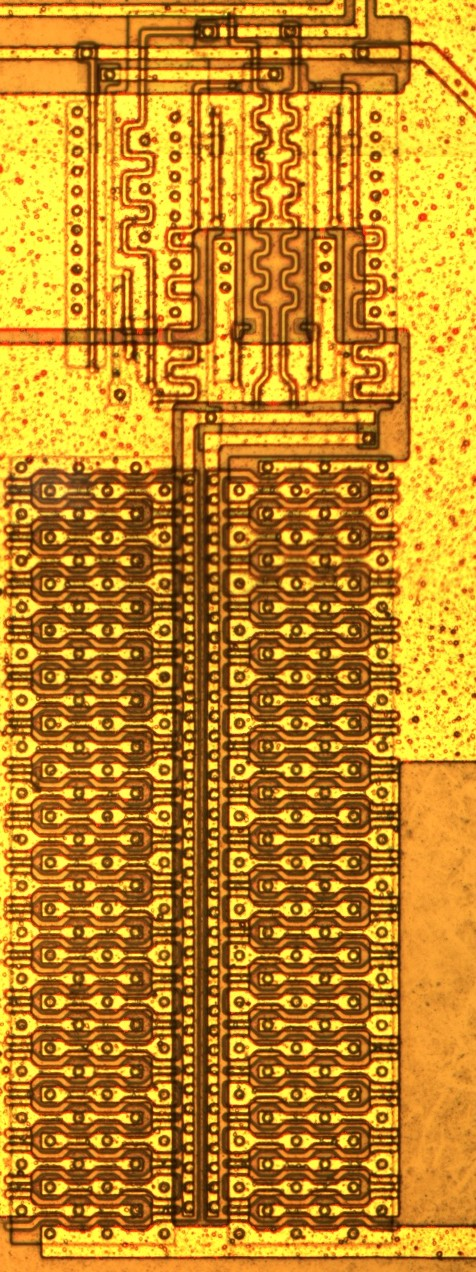
\includegraphics[height=0.95\textheight]{output-shot}
    \caption{Die photograph of the output stage}
    \label{fig:output-shot}
\end{figure}

\begin{figure}
    \centering
    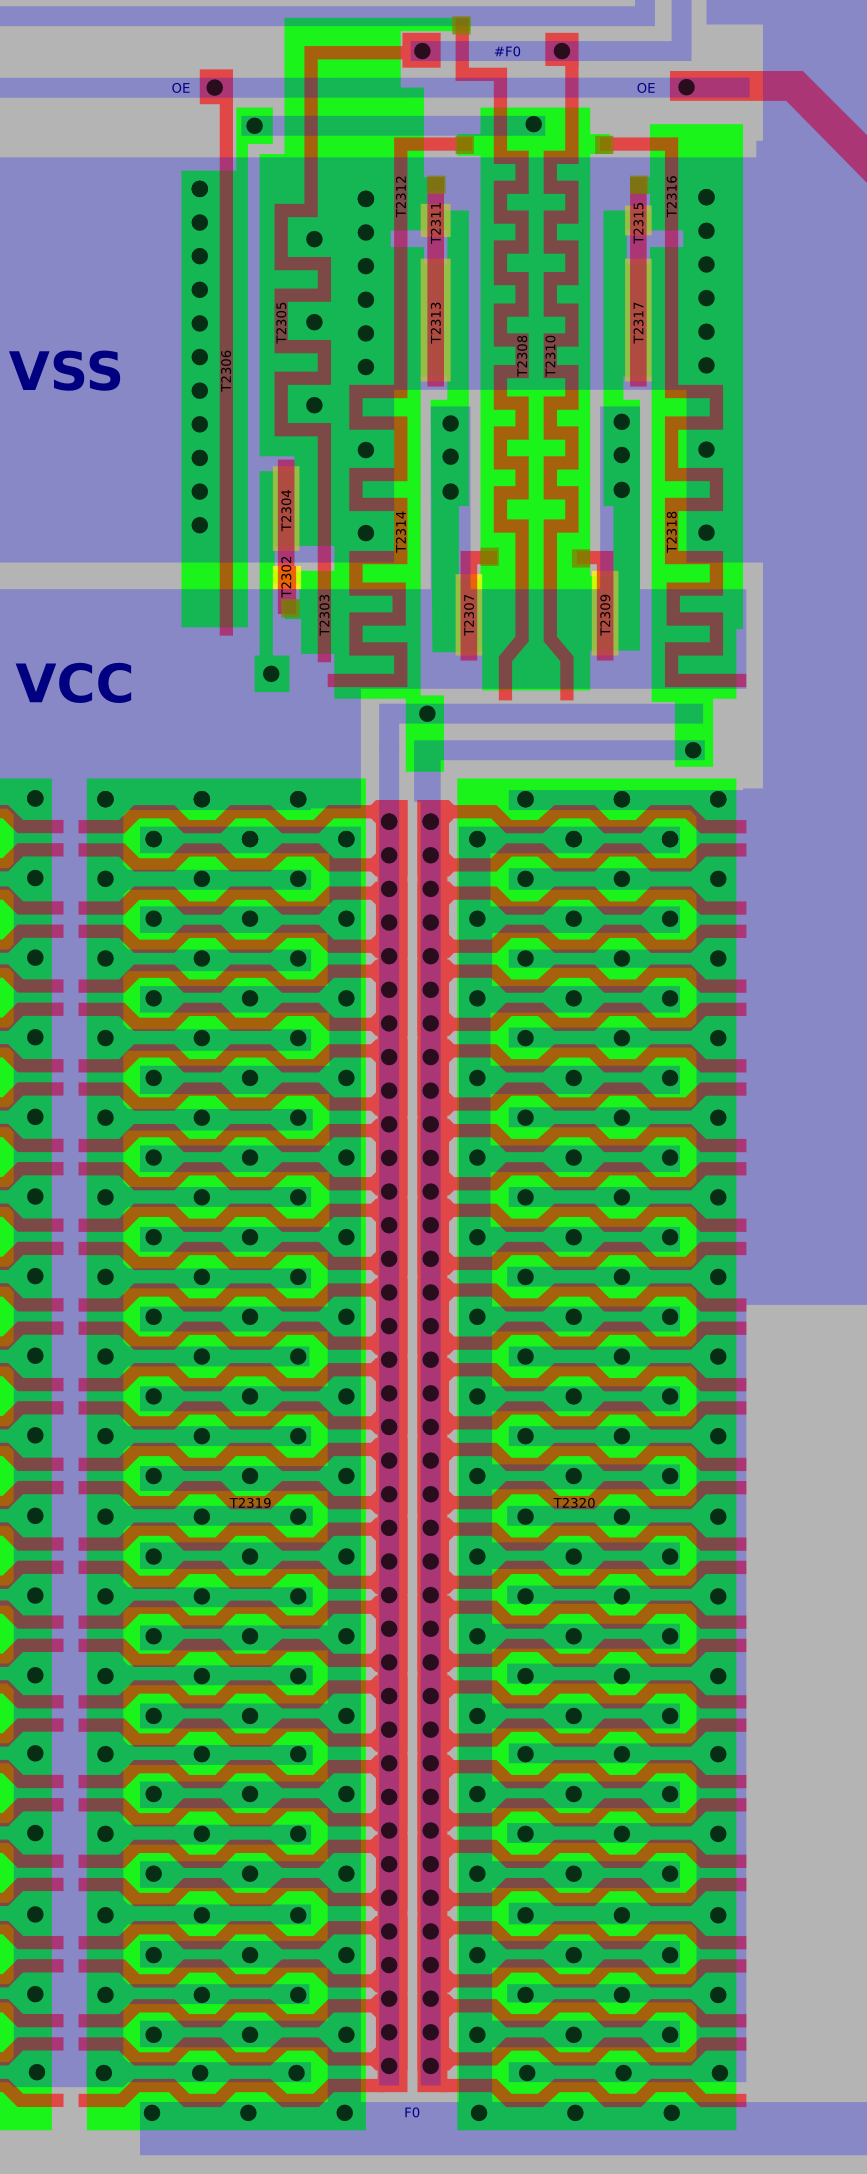
\includegraphics[height=0.95\textheight]{output-layout}
    \caption{Layout of the output stage}
    \label{fig:output-layout}
\end{figure}

\begin{figure}
    \centering
    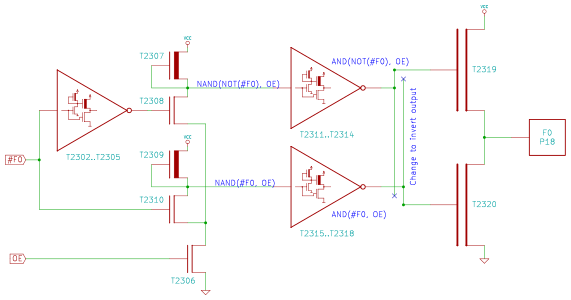
\includegraphics[width=\myupto{16cm}]{output-schem}
    \caption{Schematic of the output stage}
    \label{fig:output-schem}
\end{figure}


\begin{mytextframe}{.9\textwidth}

\textbf{Why did the initials disappear?}
People who worked on reverse engineering CSG chips noticed that older chips
usually have the initials of their engineers written on it. Later revisions
do not have these nice signatures anymore.  A certain incident was the reason.

In about 1984 or 1985 several chips were redrawn for the HMOS2 process to
reduce cost. Bret Raymis worked on a shrink of the SID chip from 6 to 5
micron. He recalls, ``I almost got fired for putting my initials on the chip
with it appearing in 3 spots across the die with `Dave's\footnote{referring
to Dave DiOrio} Bar and Grill'. The SID had three identical large blocks
with a hole in the middle.'' Dave DiOrio confirms this story, ``It actually
got fab'ed and the mask shop went berserk.''

Bret's intention was to make a joke, ``But the president of Commodore did
not think it was funny. Fortunately Mike [Angelina] took the heat and I did
not get fired.'' The chip in question was the 8580 R1 most likely.
Unfortunately only later revisions have been seen up to now, which do not
carry this Easter egg anymore.

James Redfield concludes, ``And from that day on we were no longer permitted
to include our initials on the chips.''

\end{mytextframe}

\clearpage
\section{Back-Gate Bias Generator}

The HMOS1 and HMOS2 processes used to make the PLAs use a back-gate bias
generator to adjust the FET threshold voltage. Due to the body effect the
threshold voltage of NMOS devices increases when the body voltage drops.
The back-gate bias generator consists of an oscillator and a charge pump.

The ring oscillator consists of three inverters, T2462/T2463,
T2458..T2461 and T2465/T2466. The oscillation frequency is limited by two RC
low-pass filters, T2464/C3 and T2467/C2. The totem pole T2456, T2457 and C1
form the charge pump. The two FETs T2454 and T2455 function like diodes for
the charge pump.

Figure \ref{fig:bias-spice} show a simulation of this circuit. The actual
voltages and the oscillation frequency depend from the process parameters.
As most of the parameters are not known, this simulation is only useful to
show the working principle.

\begin{figure}
    \centering
    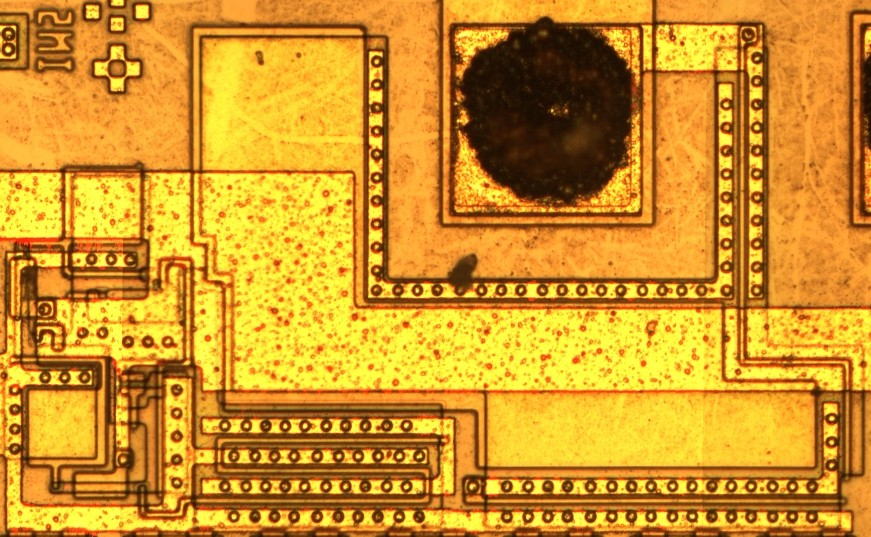
\includegraphics[width=\myupto{18cm}]{bias-shot}
    \caption{Die photograph of the back-gate bias generator}
    \label{fig:bias-shot}
\end{figure}

\begin{figure}
    \centering
    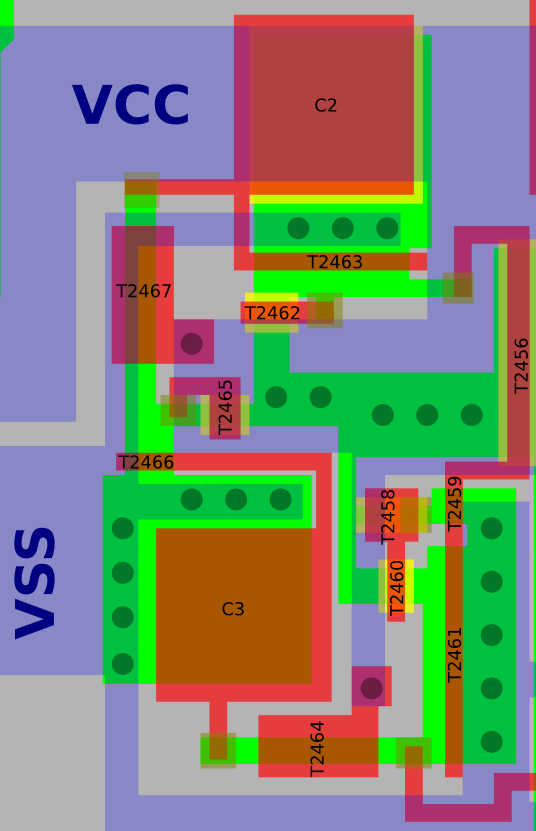
\includegraphics[width=\myupto{7cm}]{bias-layout1}
    \caption{Layout of the back-gate bias generator (oscillator)}
    \label{fig:bias-layout1}
\end{figure}

\begin{figure}
    \centering
    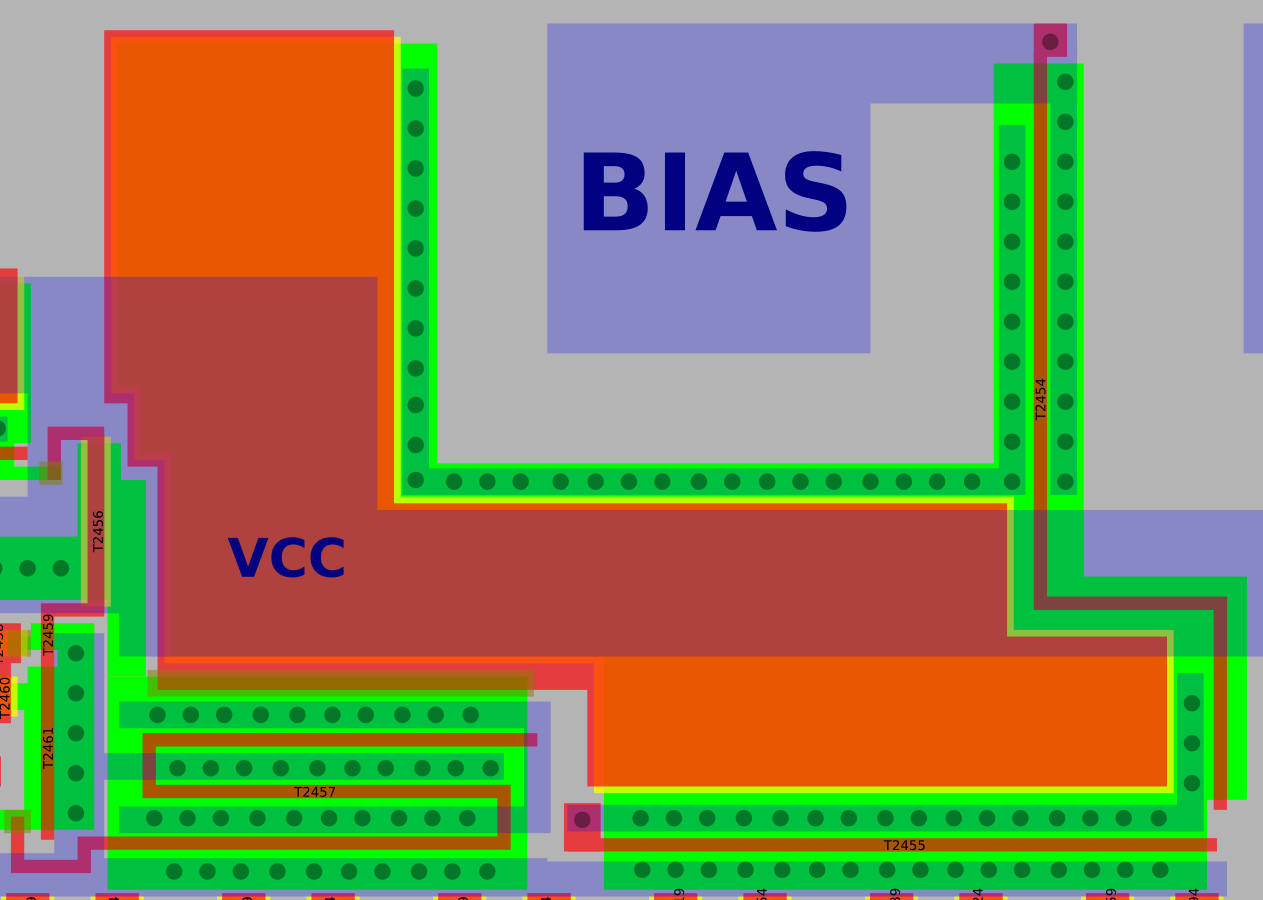
\includegraphics[width=\myupto{18cm}]{bias-layout2}
    \caption{Layout of the back-gate bias generator (charge pump)}
    \label{fig:bias-layout2}
\end{figure}

\begin{figure}
    \centering
    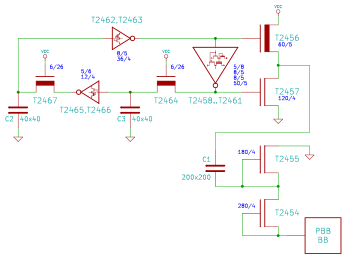
\includegraphics[width=\myupto{16cm}]{bias-schem}
    \caption{Schematic of the back-gate bias generator}
   \label{fig:bias-schem}
\end{figure}


\begin{figure}
    \centering
    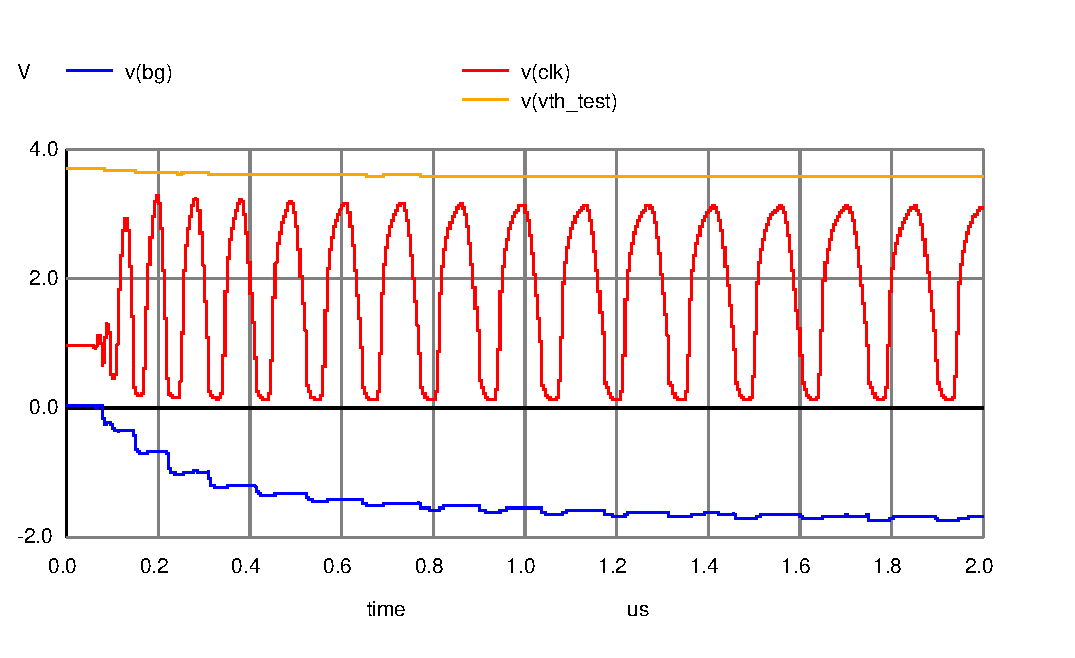
\includegraphics[width=\myupto{17cm}]{bias-spice}
    \caption{SPICE simulation of the backgate bias generator}
    \label{fig:bias-spice}
\end{figure}

\clearpage
\section{List of Components}

Table \ref{tab:pla-components} shows the list of transistors, resistors and
capacitors found on an MOS 8700R1 and their assignment to functional blocks
described in this document.

\begin{table}[h]
\begin{minipage}{\linewidth}
    \tabletextsize
    \centering
    \begin{tabularx}{\mywidthfull}{c|X}
        \toprule
        Annotation & Part usage \\
        \midrule
        R1..R16         & Part of ESD protection for inputs I0..I15 \\
        T1..T208        & ESD protection, input buffer and
                          inverter for inputs I0..I15 \\
        R17             & Part of ESD protection for OE input \\
        T209..T213      & ESD protection and input buffer for OE \\
        T214..T1893     & NOR array for product terms, only some
                          transistors actually populated \\
        T1894..T2301    & NOR array for sum terms, only some
                          transistors actually populated \\
        T2302..T2453    & Output stage and pad push-pull pad buffers \\
        T2454..T2467,
        C1..C3          & Back-gate bias generator \\
        \bottomrule
    \end{tabularx}
    \caption{List of components on 8700R2 chip}
    \label{tab:pla-components}
\end{minipage}
\end{table}


\chapter{A PLA Replacement: realPLA}
\label{sec:realpla}

The realPLA is a PLA replacement which I developed with the results of the
investigations shown in this document. It was developed with the aim to work
with all C64s which work with original PLAs too. It uses only parts which are
still in production and available at low cost as the time of writing.

The logic functions are implemented in a Lattice LC4032V CPLD. Although it
runs at 3.3 Volts, it is 5 Volt tolerant. Because of this property the CPLD
inputs can be connected to the PLA inputs directly. They even have an input
threshold voltage which is quite close to the one of the CSG PLAs.

The logic programmed to the CPLD has been converted from the JEDEC file
converted from a 82S100 to VHDL with a small Python tool. The CASRAM
equation does not fit into one macrocell of this CPLD, because it either has
too many inputs or it needs to use feedback from other terms. To provide
matching propagation delays for all input to output paths, all terms have
been edited to use two levels of logic. A binary PLA dump has been used to
execute a unit test for the logic part of this PLA implementation.

In addition to the logic functions of the PLA, also the dynamic
characteristics have to be similar to the original parts, mainly propagation
delay and slew rates.

It would have been possible to increase the propagation delay of the CPLD by
using additional internal nodes. However, as the speed grade of the CPLD may
vary and also depends on factors like temperature, this was not the way
chosen. Instead an RC delay has been added for each channel, plus a Schmitt
trigger to get well-defined edges again. The RC delay has been dimensioned
to get an overall propagation delay as an average original PLA. Finally each
output incorporates a serial resistor to limit its slew rate. The Schmitt
trigger which also translates the voltage from \SI{3.3}{\volt} to \SI{5}{
\volt} has the additional positive effect that high to low transitions are
slightly more delayed than than low to high transitions, which completely
inhibits any chip select overlap.

The PCB has been designed to have nearly the same size as an original DIP-28
PLA. This allows it to fit in all C64s, even if there is e.g., a heat sink
attached to adjacent chips.

The design of the realPLA is licensed under Creative Commons
Attribution-ShareAlike 3.0 Unported (CC BY-SA 3.0). The design files are
available at \url{https://bitbucket.org/skoe/pla}.
Figure \ref{fig:realpla-schem} shows the schematic diagram of realPLA.


\begin{figure}
    \centering
    \includegraphics[width=\myupto{10cm}]{realpla-c64}
    \caption{The realPLA}
    \label{fig:realpla-c64}
\end{figure}


\begin{sidewaysfigure}
\centering
\scalebox{0.8}{\includegraphics{realpla-schem}}
\caption{realPLA schematic diagram}
\label{fig:realpla-schem}
\end{sidewaysfigure}


\chapter{Conclusion}
\label{sec:conclusion}

There have been numerous discussions about the PLA and its properties in the
past. The reason may have been bad PLA replacements which did not work on
all C64s or not with all hardware extensions. The full logic of the PLA was
not officially documented by Commodore, which made it necessary to reverse
engineer it to be able to implement advanced programs or hardware
extensions. In contrast to the CPU, which was of interest for every
assembler programmer, the PLA was only examined by a few people. This is
another point which made the PLA look somewhat intransparent.

However, this document shows that there is no such obscurity and that most
of its properties have been found years ago already. Others can be measured
easily or can be derived from C64 schematics. The logic incorporated in the
PLA is shown in different comprehensive ways. With the hardware facts
presented in this document it is easy to see what the important requirements
for a compatible PLA replacement are. It also helps to identify properties
of PLA replacements which could make it incompatible to certain boards.

Programmable memory devices (PROMs, EPROMs) have frequently been used to
replace PLAs. The idea to do this is reasonable, a PLA is a device with a
programmable AND array followed from a programmable OR array, while a PROM
is a device with a fixed AND array\footnote{The address decoder}, and a
programmable OR array. One must be aware that a PLA replacement has to
comply with the requirements of a narrow timing window to work with all
boards, no matter if it is made using programmable logic devices or
programmable memory. Additionally, the timing printed on the chip is usually
not the typical delay which counts here. Note that programmable logic
devices usually have a very well defined and documented timing behavior,
while PROMs may have different propagation delays for different address
lines, caused by their internal geometry in rows and columns. So it is
acceptable to use a PROM as PLA replacement, as long as the actual timing
has been verified accurately.

The SuperPLA has been the first professional PLA replacement. It is known to
work on nearly all boards. Yet, it happens to fail on a few C64 boards with
a \textit{KU} serial number. This board revision is infamous for its fragile
timing. Reasons for the failures are hard to identify. It may be caused by
the not fully authentic timing or by the fast slew rates which even caused
undershoots in the measurements.

The EPROM PLA replacement M27C512-90B6 is one of the simplest PLA
replacements. Recalling the bad experience some people had with the
compatibility of other EPROM PLA replacements it was highly controversial.
However, the sample tested in this document made a good impression. The only
negative point seen was the slightly too fast propagation delay, which is
most likely the reason that it also failed with a few KU boards.

The prototypes of the realPLA have been tested on about 20 C64 boards of
different board revisions, including KU boards. The compatibility of the
realPLA with different C64 expansions has been checked, for example
EasyFlash 3 and Turbo Chameleon. The realPLA worked on all of these boards.
However, there can never be a guarantee that a PLA or PLA replacement works
on absolutely every board with any extension ever designed. The different
lots and revisions of C64 computers with different VIC-II chips have
different timing requirements, which was also known to Commodore: They
defined different RC delays for different combinations.

The chapter which describes the reverse engineering and inner workings of a
CSG PLA may be of less practical interest. It is more focused on
understanding how this part was developed and how it works, for educational
and historical purposes.

Hopefully this document can help other hardware projects, emulators and
programmers to improve and prolong the experience with the definitely best
computer of the world ;)


%%%%%%%%%%%%%%%%%%%%%%%%%%%%%%%%%%%%%%%%%%%%%%%%%%%%%%%%%%%%%%%%%%%%%%%%
\appendix

\chapter{C64 Memory Configurations Explained}
\label{sec:memmaps}

The Commodore 64 memory configurations are explained in various books and
other documents. Some of these tables are incomplete or even flawed.

For the sake of completeness of an C64 PLA article they are listed here once
more. All tables have been generated directly from the JEDEC file read out
from a 82S100 PLA, so it is very unlikely that there are mistakes in them.

There is a mechanism implemented in the PLA logic which is not shown in the
tables below. Section \ref{sec:connection} explains how
the VIC-II can halt the CPU when it wants to take over the bus. If write
accesses by the CPU address the I/O area during this phase, the PLA selects the
I/O chips accordingly. But to make sure that the (dummy) read cycles in this
phase will never accidentally acknowledge an interrupt, the PLA redirects them
to RAM. The signals BA and R/\#W are used to identify this situation.

Jens Schönfeld's PLA analyzer is useful to explore the C64 memory maps
interactively. It can be downloaded at
\url{http://icomp.de/products/SuperPLA/pla_analyzer.zip}. It runs in a DOS box,
also in the DOS emulator \textit{dosbox} under Linux.

\input{obj/memtabs.tex}

%%%%%%%%%%%%%%%%%%%%%%%%%%%%%%%%%%%%%%%%%%%%%%%%%%%%%%%%%%%%%%%%%%%%%%%%
% http://tim.thorpeallen.net/Courses/Reference/Citations.html

\begin{thebibliography}{999}
\input{obj/bibliography.tex}
\end{thebibliography}

\end{document}

